%
% main.tex -- Paper zum Thema "Extreme Ereignisse"
%
% (c) 2018 Melina Staub, Hochschule Rapperswil
%
\chapter{Extreme Ereignisse\label{chapter:thema}}
\lhead{Extreme Ereignisse}
\begin{refsection}
\chapterauthor{Melina Staub}


\section{Einleitung}
Fast täglich erscheinen Schlagzeiten wie diese in der Zeitung:

\begin{itemize}
\item Wetter-Extreme häufen sich auch in der Schweiz
\item Seit Lothar wird es der vielleicht stärkste Sturm
\item Die Schweiz reagiert empfindlich auf Wetteränderung
\item Unwetter sorgten für eine chaotische Nacht
\item Schweiz besonders stark vom Klimawandel betroffen
\end{itemize}

Doch wieviel Wahrheit steckt in diesen Headlines? Sind sie nur Hirngespinste der Nachrichtenindustrie? Wollen uns die Medien täuschen oder geht da draussen wirklich etwas vor sich?

Dass die Natur im Wandel ist, steht ausser Frage. In der Geschichte der Erde waren extreme Ereignisse keine Seltenheit. Ob Eiszeiten, Trockenperioden oder lang anhaltende Regenschauer, wohl jedes vorstellbare Ereignis ist vorgekommen. Vulkanausbrüche pumpten Kohlendioxid in die Atmosphäre und Meteoriteneinschläge lösten Tsunamis aus, welche die Landflächen fluteten. Die Erde hat sich von Zeit zu Zeit und nach jedem Ereignis erholt oder angepasst. Doch seit Mitte des 18. Jahrhunderts mit der Industrialisierung hat sich viel verändert.

Die nachfolgenden Seiten wurden ohne Vorurteile oder frühzeitigen Feststellungen rund um den Klimawandel erstellt. Am Ende soll die Wahrheit festgestellt werden.
Was bereits klar ist, die Erde wird den Klimawandel überstehen, wie sie auch schon extreme Trockenperioden oder Eiszeiten überlebt hat. Doch was aus uns?


\section{Was sind extreme Ereignisse?}
Die Diskussionen um den Klimawandel erregt die Gemüter auf der ganzen Welt. Einige verleugnen ihn und andere verstehen ihn und tun alles um ihn zu stoppen. Besonders extreme Ereignisse wie starke Regenfälle und die daraus resultierenden Überschwemmungen und Verwüstungen bleiben uns stark in Erinnerung.
Eben diese Ereignisse weichen stark von den Durchschnittswerten ab und hinterlassen oft grosse Schäden und ebenso grosse Schadensummen. Doch nicht nur überdurchschnittlich starke Ereignisse, sondern auch sehr kleine wie Trockenperioden oder Wasserknappheit sind extreme Ereignisse.
Jetzt stellt sich die Frage, ob diese extremen Ereignisse natürlichen Ursprungs sind, also  die Anordnung durch den Zufall bestimmt wird und auch ohne den Einfluss des Menschen passiert wären oder ob diese auf den Klimawandel zurückzuführen sind und somit eine unnatürliche Häufung aufzeigen.


\subsection{Aufzeichnungen in der Schweiz}
In den \textit{Schweizer Wetterjahresbücher} und \textit{Analen der Schweizerischen Meteorologischen Zentralanstalt} lassen sich Wetter- und Klimadaten bis ins Jahr 1864 abrufen. Umfangreiche Tabellen und Berichte sind für Wetter- und Klimainteressierte ein historisch sehr bedeutender Datenschatz. 
Der Monatliche Wetterverlauf wurde ab dem Jahr 1911 geführt, extreme Wetterereignisse in Berichten beschrieben und aufgezeichnet (Abbildung \ref{Analen}). Die Analen wurden 2011 durch den Klimareport abgelöst, seit diesem Jahr sind der Klimabericht wie auch die Analen für die Öffentlichkeit zugänglich und können Online eingesehen werden.
Mit diesen langen und genauen Klimadaten lässt sich tief in die Vergangenheit des Schweizer Klimas blicken. Ein Blick in die Klima-Vergangenheit wird möglich.

\begin{figure}
\centering
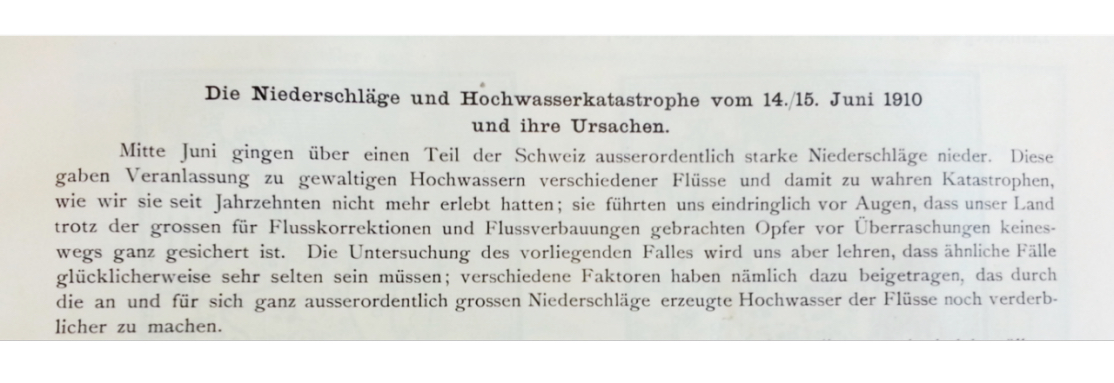
\includegraphics[width=\hsize]{extrem/Analen.jpg}
\caption{Originaltext aus den Annalen 1910 zur Hochwasserkathastrophe vom Juni 1910. (Quelle: MeteoSchweiz)}
\label{Analen}
\end{figure}


\subsection{Homogene Messreihen}
Um die Klimadaten der letzten 150 Jahre miteinander zu vergleichen, müssen die Messergebnisse vor dem Vergleich homogenisiert werden (Abbildung \ref{Homogen}). Die Modernisierung der Messgeräte,  eine Verschiebung des Messstandortes oder die Veränderung der Umgebung führen zu anderen Messwerten als beispielsweise diese des Vorgänger Messgeräts. Die Daten liefern einen verfälschten Vergleich, wenn man sie ohne Homogenisierung miteinander vergleicht.
Wenn man den Messstandort verlegt, verändert sich die Höhenlage. Dies wirkt sich auf die Temperaturmessung aus, da sich diese mit der Höhe im Mittel verschiebt. Die Messreihe wird ungenau und ein verfälschtes Bild zeichnet sich ab, welches nichts mit dem Klima zu tun hat.
Um diese Fehlinterpretationen zu vermeiden, sind in den \textit{Schweizer Wetterjahresbücher} und \textit{Analen der Schweizerischen Meteorologischen Zentralanstalt} sämtliche Messwerte homogenisiert worden. Ein direkter Vergleich ist nun möglich.

\begin{figure}
\centering
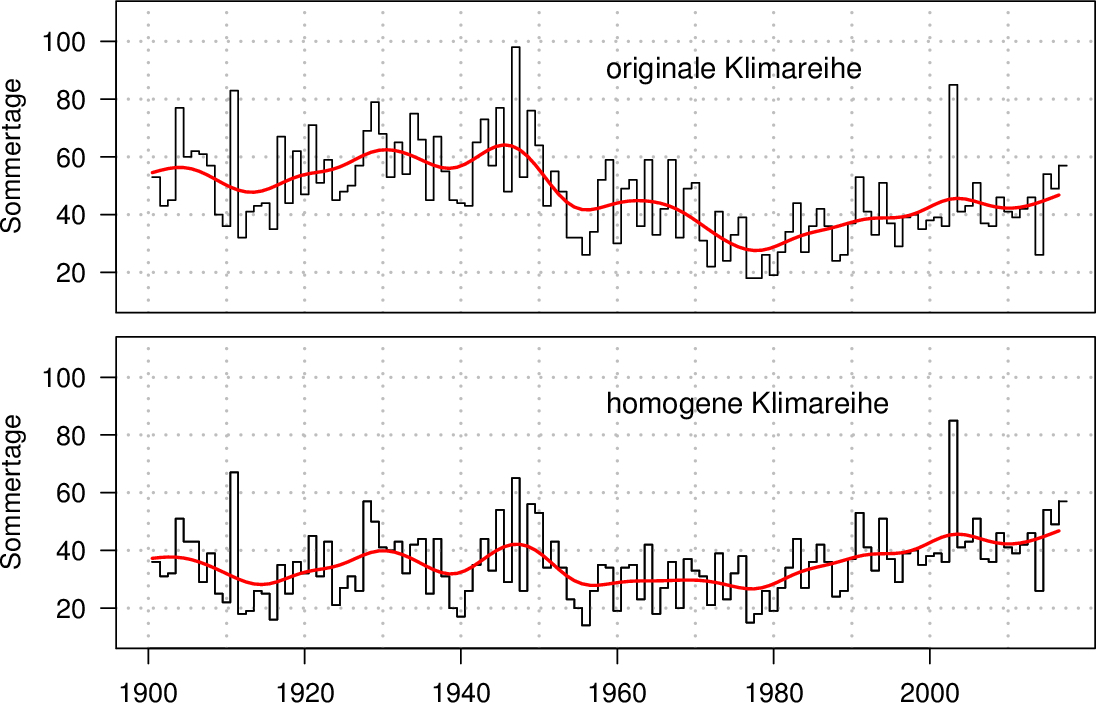
\includegraphics[width=0.6\textwidth]{extrem/Homogen.jpg}
\caption{Entwicklung der Anzahl Sommertage (Maximum--Temperatur $\ge 25^{\circ}$C ) pro Jahr an der Messstation Zürich/Fluntern seit 1901, gerechnet aus der originalen und homogenen Temperatur--Messreihe. Der geglättete Verlauf ist rot eingezeichnet. (Quelle: MeteoSchweiz)}
\label{Homogen}
\end{figure}


\section{Unwetterlotto}
Um herauszufinden ob extreme Ereignisse nicht durch den Zufall bestimmt werden, benötigen wir vorerst ein Modell um diese Berechnungen durchführen zu können.
Hierbei bedienen wir uns dem Glücksspiel, genauer gesagt dem Lotto.

\begin{figure}
\centering
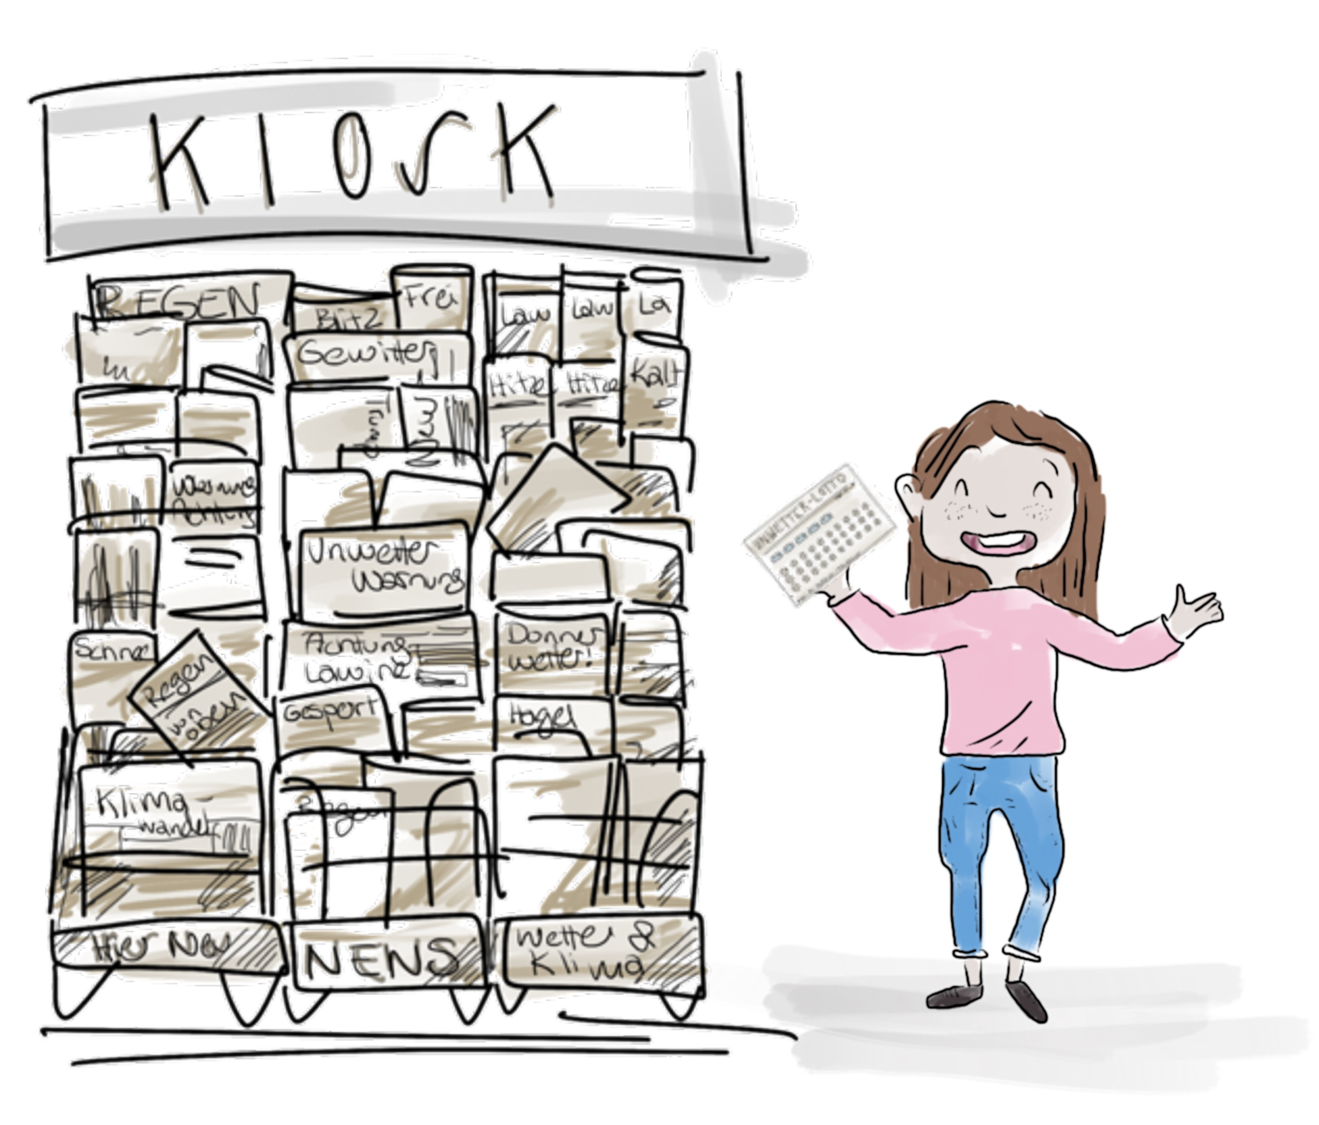
\includegraphics[width=0.4\textwidth]{extrem/Kiosk.pdf}
\caption{Unwetterlottoschein exklusiv erhältlich für Mathsem Teilnehmer.}
\label{Kiosk}
\end{figure}

Exklusiv für die Leserinnen und Leser dieses Seminarbuches steht der Unwetterlottoschein zur Verfügung, welchen man am Zeitungskiosk (Abbildung \ref{Kiosk}) erwerben und statt auf Zahlen auf Unwetterereignisse tippen kann. Auf dem Unwetter-Lotto-Schein (Abbildung \ref{Lottoschein}) kann wie beim normalen Zahlenlotto aus verschiedenen Zahlen ausgewählt und seine Tipps abgeben werden. Danach gibt es eine Unwetterziehung und man kann seine abgegebenen Tipps mit der Ziehung vergleichen.

\begin{figure}
\centering
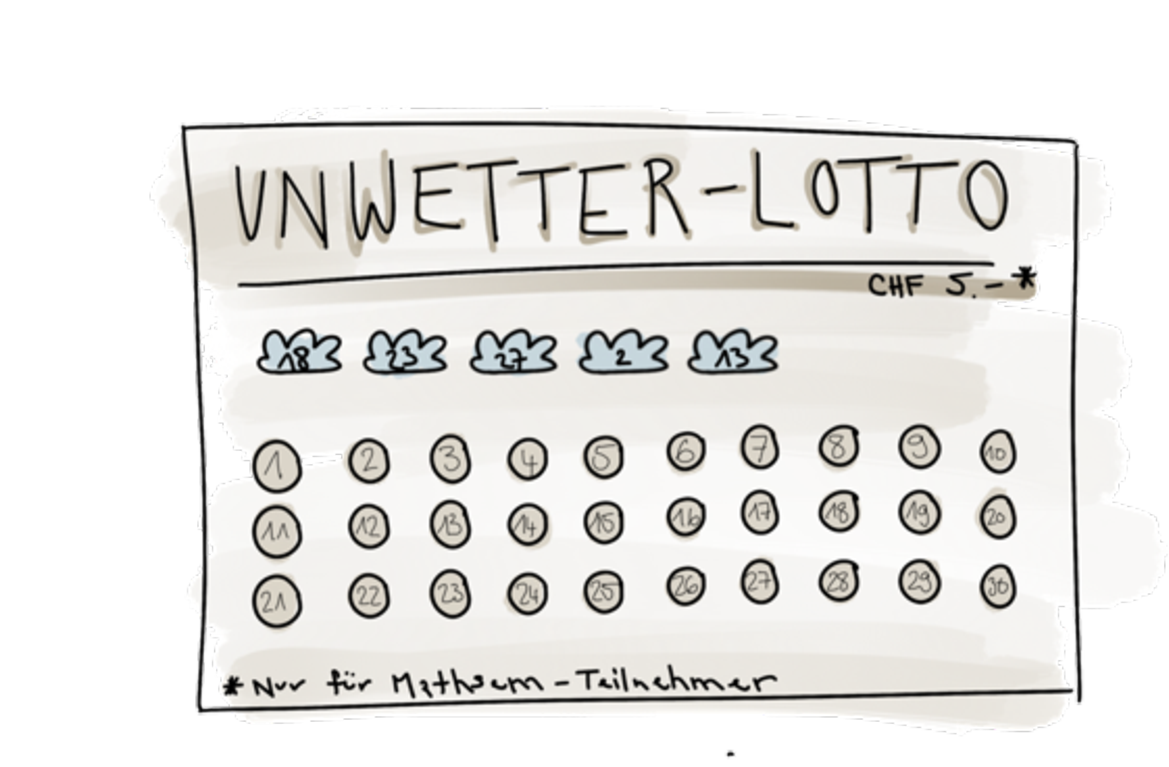
\includegraphics[width=0.7\textwidth]{extrem/Lottoschein.pdf}
\caption{Unwetterlottoschein.}
\label{Lottoschein}
\end{figure}

Die Kugeln 1-30 beschreiben alle vorhandenen Ereignisse, welche wir \textcolor{red}{\textbf{N}} nennen. Die fünf Wolken stehen für die Anzahl Tipps (Kreuze), welche wir abgeben dürfen. Das heisst, welche Unwetter \textcolor{blue}{\textbf{n}} wir aus den totalen Ereignissen 1-30 auswählen können. Die bei der Unwetterziehung gezogenen Ereignisse \textcolor{green}{\textbf{M}}, sind unsere Stichproben aus allen Ereignissen (Abbildung \ref{ErklaerungLotto}).

Jetzt stellen wir uns die entscheidende Frage: 
Wie wahrscheinlich ist es, ein 5er im Unwetter-Lotto (Abbildung \ref{WahrscheinlichkeitUnwetterlotto})zu erhalten? Diese Wahrscheinlichkeit bezeichnen wir mit \textcolor{yellow}{\textbf{k}}.

\begin{figure}
\centering
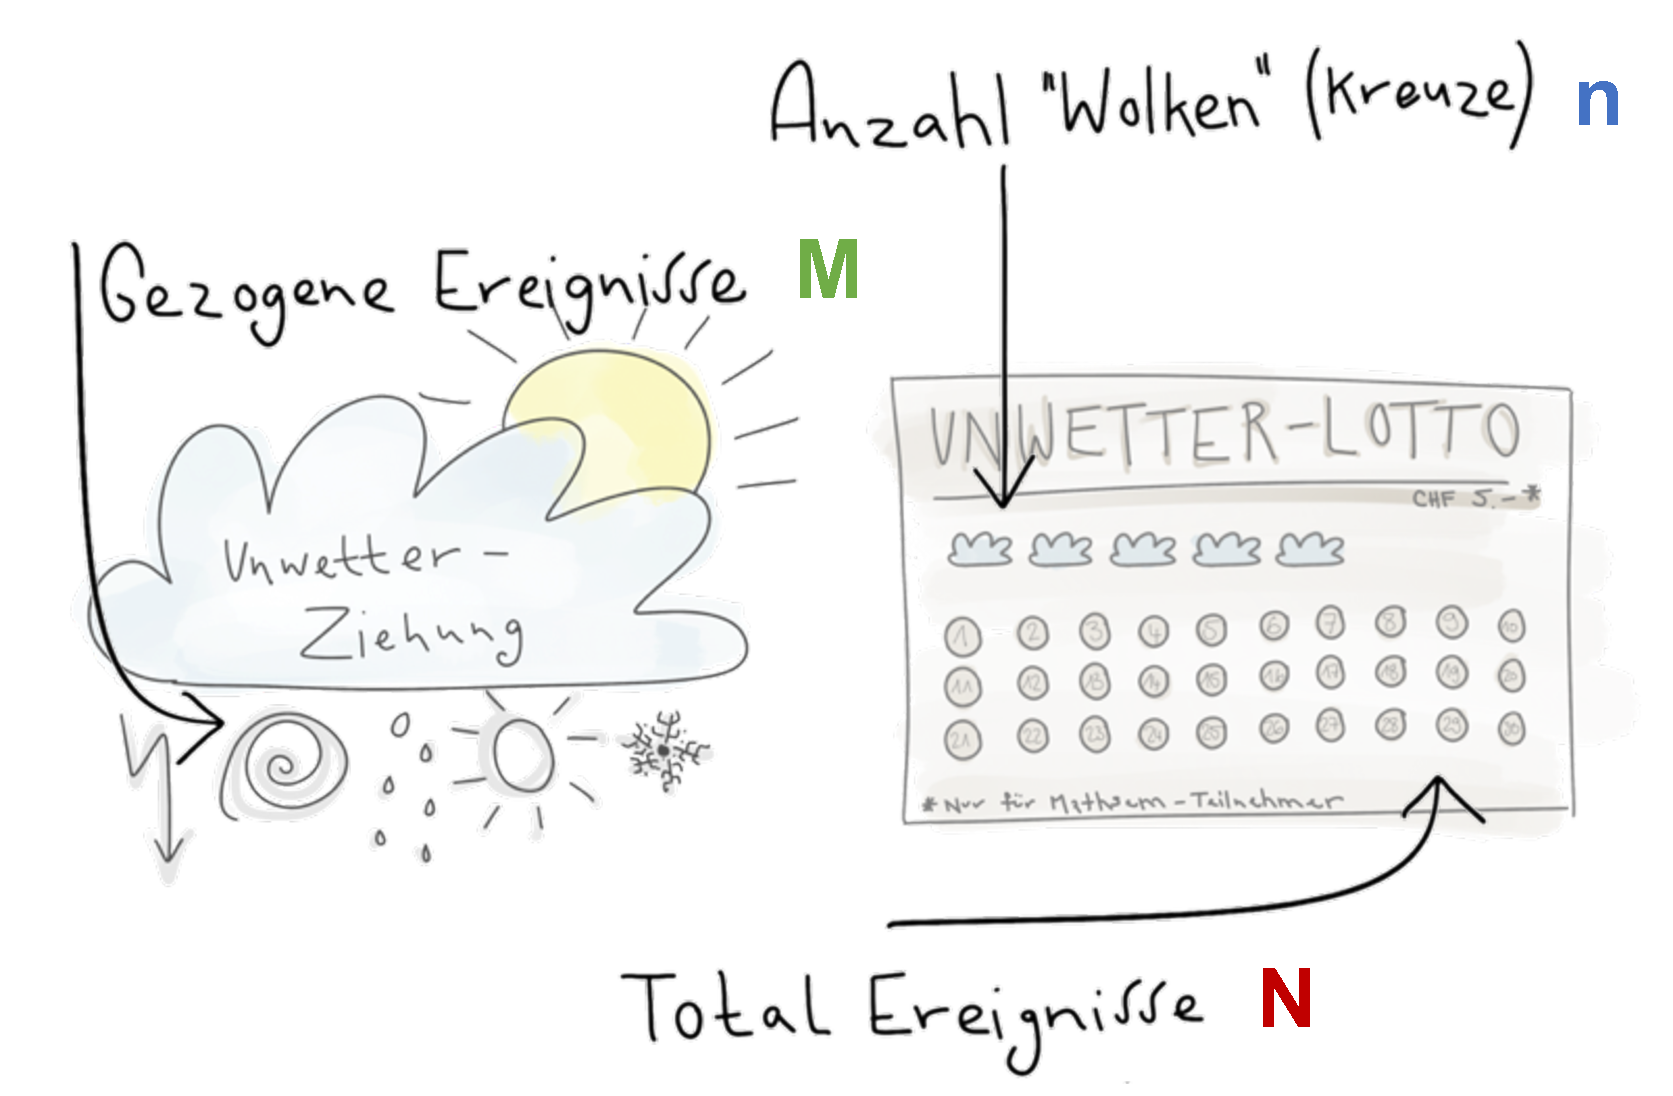
\includegraphics[width=0.6\textwidth]{extrem/Lottoscheinausgefuellt.pdf}
\caption{Unwetterlottoschein mit den Variabeln und der Unwetterziehung.}
\label{ErklaerungLotto}
\end{figure}

\begin{figure}
\centering
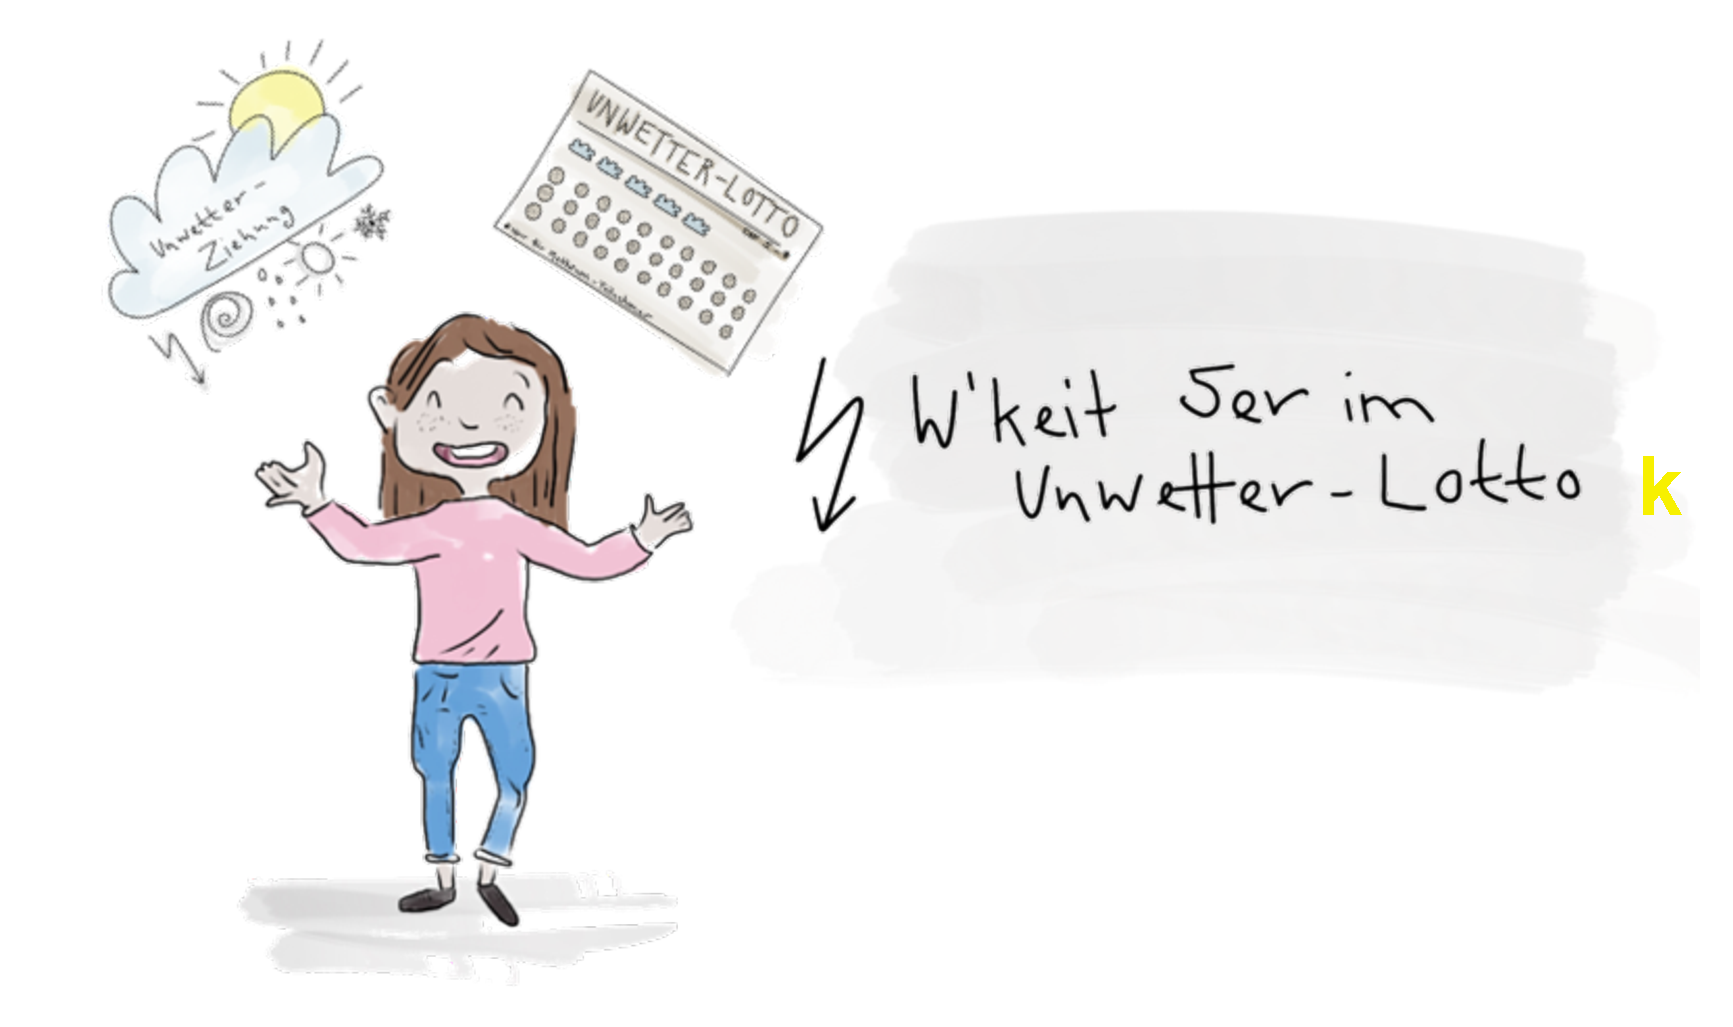
\includegraphics[width=0.6\textwidth]{extrem/wkeitlotto.pdf}
\caption{Wahrscheinlichkeit, einen 5er im Unwetterlotto zu erhalten.}
\label{WahrscheinlichkeitUnwetterlotto}
\end{figure}


\subsection{Lottoproblem} \label{Lottoproblem}
Mit dem Unwetterlotto wurde das bekannte Lottoproblem beschrieben - ein Experiment ohne zurücklegen. Mit jeder Ziehung ändert sich im Laufe des Experiments die Grundgesamtheit und somit auch die Wahrscheinlichkeit ein bestimmtes Ereignis zu ziehen. Der Ziehmodus ist vorgegeben und somit ist auch der Gewinn bekannt.
Das oben beschriebene Lottoproblem liefert uns folgende Fragestellung:


Wie wahrscheinlich ist es...

\begin{itemize}
\item \dots auf einem Lottozettel mit \textcolor{red}{\textbf{N}} Feldern \dots
\item \dots auf welchem man \textcolor{blue}{\textbf{n}} Unwetter ankreuzen kann \dots
\item \dots und bei der Ziehung \textcolor{green}{\textbf{M}} Unwetter gezogen werden \dots
\item \dots genau \textcolor{yellow}{\textbf{k}} Richtige zu haben?
\end{itemize}


\section{Die Unwetter-Verteilung}
Um die Frage zu beantworten, ob sich das Klima verändert und ob immer häufiger extreme Ereignisse auftreten, bedienen wir uns aus dem Werkzeugkasten der Statistik. Mit dem genannten ~\ref{Lottoproblem} \nameref{Lottoproblem}, lässt sich die Unwetter-Verteilung aufstellen. Die Fragestellung muss dabei ein wenig auf unser Problem angepasst werden.

Dabei beziehen sich die \textcolor{red}{\textbf{N}} Felder auf dem Lottozettel auf die Anzahl Jahre mit zugehörigen Messwerten. Die Anzahl Unwetter \textcolor{blue}{\textbf{n}} welche man ankreuzen kann, sind die extremen Ereignisse, also Unwetter oder Messungen welche besonders extrem ausgefallen sind. Die Ziehung der \textcolor{green}{\textbf{M}} Unwetter ist unser Beobachtungszeitraum. Im nachfolgenden Abschnitt ~\ref{Beispiel} \nameref{Beispiel} wird ein Beobachtungszeitraum von 10 Jahren angenommen. Die Frage welche nun beantwortet werden muss lautet:

Wie wahrscheinlich (\textcolor{yellow}{\textbf{k}}) ist es, dass \textcolor{blue}{\textbf{n}} extreme Ereignisse aus einer Messreihe von \textcolor{red}{\textbf{N}} Jahren, in den letzten 10 Jahren (\textcolor{green}{\textbf{M}}) vorkommen? 


\begin{figure}
\centering
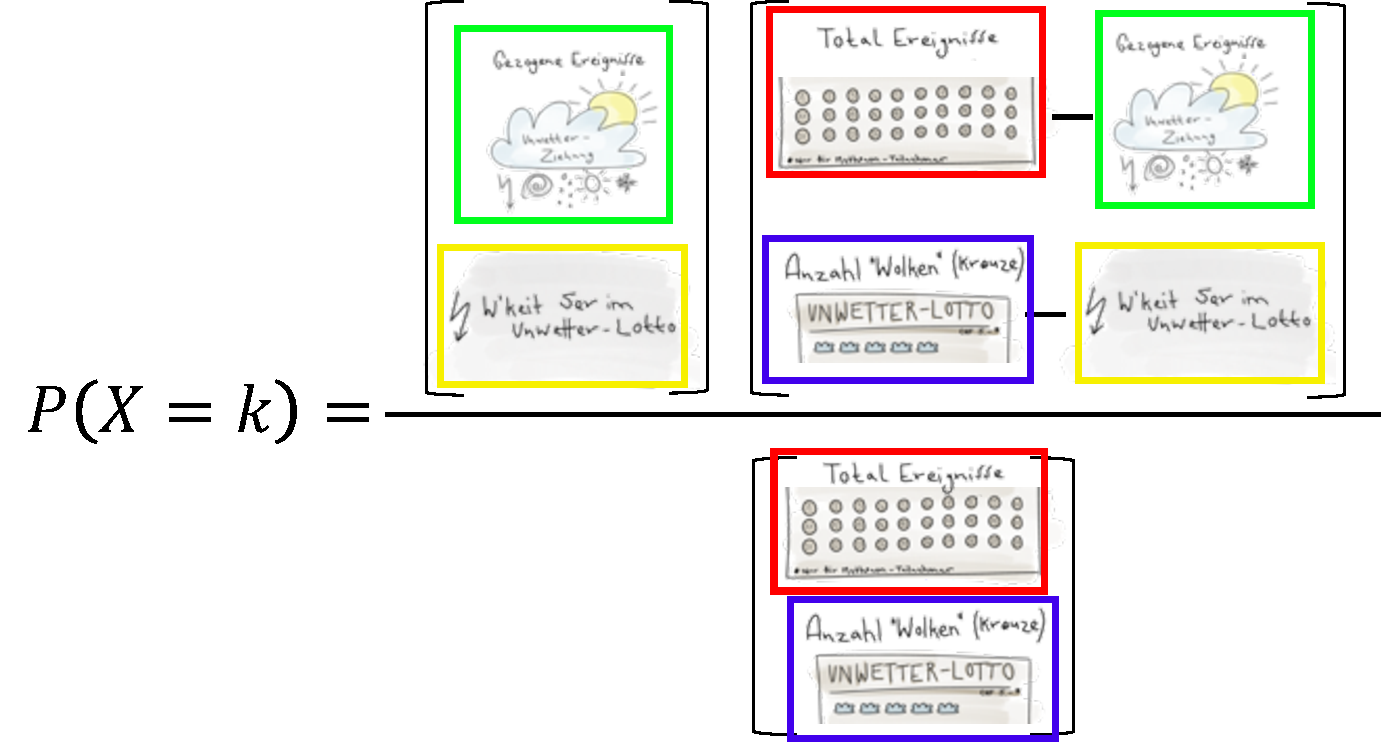
\includegraphics[width=0.6\textwidth]{extrem/Unwettervert.pdf}
\caption{Die Unwetter-Verteilung. Die Wahrscheinlichkeit sagt aus, wie wahrscheinlich es ist n extreme Ereignisse aus einer Messreihe von N Jahren in den letzten 10 Jahren (M) vorzufinden.}
\label{UnwetterVerteilung}
\end{figure}

Je tiefer die Wahrscheinlichkeit ausfällt, desto unwahrscheinlicher ist es, dass viele extreme Ereignisse in den letzten 10 Jahren (\textcolor{green}{\textbf{M}}) vorkommen. Dies ist dann der Fall, wenn die Wahrscheinlichkeit von einigen Ereignissen berechnet wird.
Die Unwetter-Verteilung ist somit nichts anderes als die hypergeometrische Verteilung \eqref{V1}. 

Die hypergeometrische Verteilung

\begin{equation}
P(X = k) = 
\frac{\displaystyle \binom{M}{k} \binom{N-M}{n-k}}{\displaystyle \binom{N}{n} } 
\label {V1}
\end{equation}

beschreibt die Wahrscheinlichkeit aus $N$ gegebenen Elementen, mit $n$ Elementen einer speziellen Eigenschaft, und einer Stichprobe aus $M$ Elementen genau $k$ Treffer zu erzielen. 
Anders als die Binomialverteilung ist die hypergeometrische Verteilung ein Experiment ohne zurücklegen. Die Wahrscheinlichkeit ändert sich mit jeder Ziehung. Die Frage wie wahrscheinlich (k) es ist, dass n extreme Ereignisse aus einer Messreihe von N Jahren in den letzten 10 Jahren (M) vorkommt, kann nun beantwortet werden.


\subsection{Beispiel} \label{Beispiel}
Die hypergeometrische Verteilung setzt sich aus verschiedenen Binomialkoeffizienten

\begin{align*}
\binom{n}{k} = \frac {n!}{k! \cdot (n-k)!} 
\end{align*}
zusammen.

Um in ~\ref{MesspunkteSchweiz} \nameref{MesspunkteSchweiz} die Klimadaten auszuwerten, werden im nachfolgenden Beispiel der hypergeometrischen Verteilung die folgenden Werte für die entsprechenden Variabeln verwendet:
\begin{align*}
N = 75 \quad \quad \quad \quad \quad \quad 
n = 7 \\
M = 10 \quad \quad \quad \quad \quad \quad 
k = 3
\end{align*}

Die Wahrscheinlichkeit P(X=3) ergibt sich aus:
Anzahl der Möglichkeiten, genau 3 extreme Ereignisse (und damit genau 4 normale Ereignisse) auszuwählen, dividiert durch die Anzahl Möglichkeiten 7 Ereignisse aus allen Ereignissen auszuwählen. Dabei gibt es
\begin{align*}
\binom{M}{k} = \binom{10}{3} = 120
\end{align*}

Möglichkeiten, genau 3 extreme Ereignisse auszuwählen.
Zudem gibt es 
\begin{align*}
\binom{N-M}{n-k} = \binom{75-10}{7-3} = \binom{65}{4} = 677040
\end{align*}

Möglichkeiten, genau 4 normale Ereignisse auszuwählen.
Da jede Möglichkeit 3 extreme Ereignisse mit jeder Möglichkeit 4 normale Ereignisse auszuwählen kombiniert werden kann, ergibt sich
\begin{align*}
\binom{M}{k} \cdot \binom{N-M}{n-k} = \binom{10}{3} \cdot \binom{75-10}{7-3} = 120 
\cdot 677040 = 81244800
\end{align*}

Möglichkeiten für genau 3 extreme und 4 normale Ereignisse auszuwählen.
Zusätzlich gibt es insgesamt
\begin{align*}
\binom{N}{n} = \binom{75}{7} = 1984829850
\end{align*}

Möglichkeiten, 7 Ereignisse aus allen Ereignissen zu ziehen.
Für k=3 erhalten wir somit die Wahrscheinlichkeit
\begin{equation}
P(X = 3) = \frac{\displaystyle \binom{M}{k} \binom{N-M}{n-k}}{\displaystyle \binom{N}{n} }  \\
= \frac{\displaystyle \binom{10}{3} \binom{75-10}{7-3}}{\displaystyle \binom{75}{7} } \\
= \frac{ 120 \cdot 677040}{ 1984829850 } = 0.0409329 
\label {V2}
\end{equation}

In 4.09 \% aller Fälle werden genau 3 extreme und 4 normale Ereignisse vorkommen. Diese Berechnung lässt sich mit allen $X=k$ durchführen, dies wird im Kapitel ~\ref{Dichtehyper} \nameref{Dichtehyper} gemacht.


\subsection{Die hypergeometrische Verteilung} \label{Dichtehyper}
Im vorangehenden Beispiel \eqref{V2} wurde die Wahrscheinlichkeit der hypergeometrischen Verteilung berechnet für $P(k = 3)$. 

\begin{definition}
Die hypergeometrische Verteilung, sind die Wahrscheinlichkeitswerte für alle P(X=k).
\end{definition}

\begin{figure}
\centering
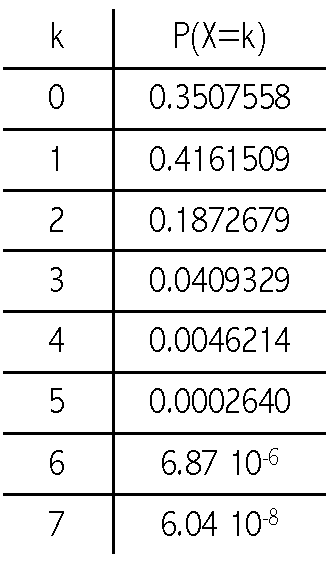
\includegraphics[width=0.2\textwidth]{extrem/TabHyperV.pdf}
\caption{Wahrscheinlichkeiten P(X=k) der verschiedenen Ereignisse, beschreiben unsere hypergeometrische Verteilung.}
\label{TabHyperV}
\end{figure}

Für alle $P (X=k)$ ergeben sich folgende Wahrscheinlichkeiten (Abbildung \ref{TabHyperV}). Die Wahrscheinlichkeit beschreibt dabei, wie wahrscheinlich es ist, genau k extreme Ereignisse in den letzten 10 Jahren vor zufinden.
Beachten Sie, dass die Werte N, M und n das Experiment beschreiben und nicht mehr verändert werden. Die Variable k hingegen kann alle möglichen Ausgänge des Experiments annehmen, in unserem Beispiel also von 0 bis 7.

\begin{figure}
\centering
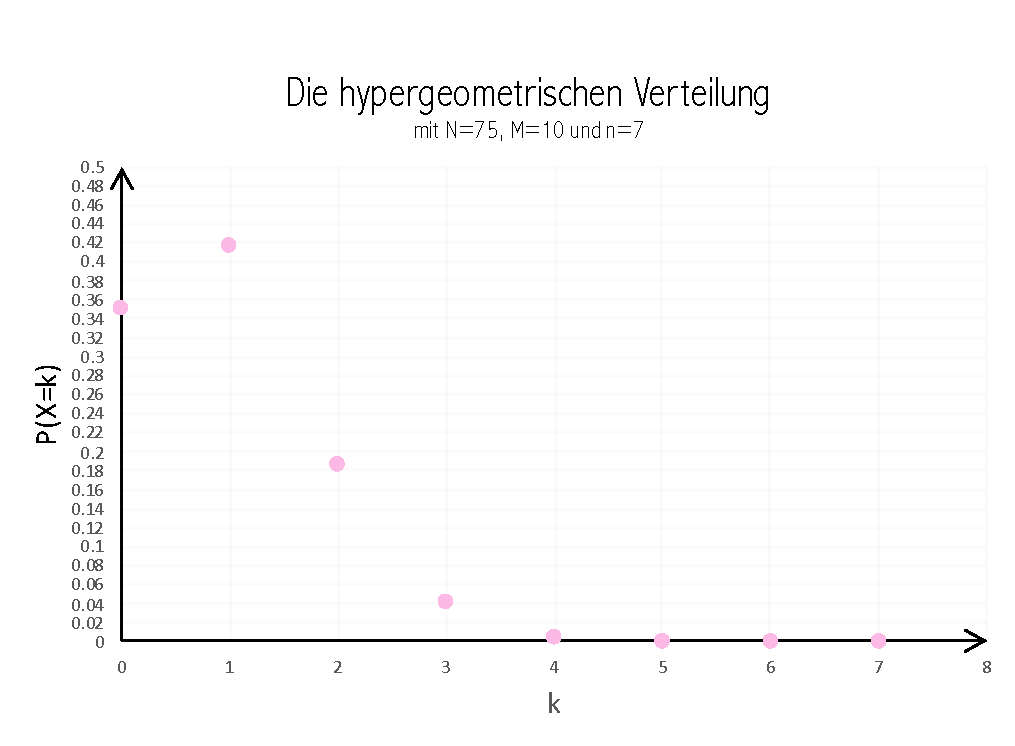
\includegraphics[width=0.8\textwidth]{extrem/HyperV.pdf}
\caption{Die hypergeometrische Verteilung unseres Beispiels. Sie zeigt auf, wie wahrscheinlich es ist, genau k extreme Ereignisse in den letzten 10 Jahren vorzufinden.}
\label{HyperV}
\end{figure}

In Abbildung \ref{HyperV} ist sehr gut ersichtlich, dass die Wahrscheinlichkeit bei genau einem extremen Ereignis in den letzten 10 Jahren am höchsten ist. Wohingegen genau 3 Ereignisse nur noch eine Wahrscheinlichkeit von 4.09\% aufweisen, was bereits sehr unwahrscheinlich ist. Häufungen von Ereignissen, welche die Anzahl 3 überschreiten, sind so unwahrscheinlich, das sie kaum natürlichen Ursprungs sein können.

\subsection{Sind viele extreme Ereignisse wahrscheinlich?}
Stellt man sich nun die Frage ob viele extreme Ereignisse wahrscheinlich sind, muss berechnet werden wie wahrscheinlich es ist k oder mehr Ereignisse in den letzten 10 Jahren (M) zu erhalten. 
Die Verteilungsfunktion der hypergeometrischen Verteilung ist nichts anderes, als die Aufsummierte Wahrscheinlichkeit aller möglichen Ausgänge. Weil für unser Beispiel aber wichtig ist, wie wahrscheinlich es ist, drei oder mehr extreme Ereignisse in den letzten 10 Jahren vorzufinden, muss die Komplementäre Verteilungsfunktion 

\begin{align*}
F(x) = P(X \ge I ) = \sum \limits_{k=I}^n P(X = k)
\end{align*}

angewendet werden (Abbildung \ref{HyperExt}). 
Möchten wir die Wahrscheinlichkeit wissen, drei oder mehr extreme Ereignisse in den letzten 10 Jahren vorzufinden, müssen die einzelnen Wahrscheinlichkeiten aufsummiert (Abbildung \ref{TabExt}) werden:

\begin{align*}
\bar{F}(3) &=  P(X {\ge} 3) \\
&= P(X = 3) + P(X = 4) + P(X = 5) + P(X = 6) + P(X = 7) \\
&= 0.0409329 + 0.0046214 + 0.00026340 + 6.87 10^{ -6 } + 6.04 10^{ -8 } \\
&= 0.045833 \quad \quad  4.58\%
\end{align*}

Drei oder mehr extreme Ereignisse in den letzten 10 Jahren sind mit einer Wahrscheinlichkeit von 4.58\% möglich. 
Die Wahrscheinlichkeit ein oder zwei extreme Ereignisse in den letzten 10 Jahren zu haben ist mit 64.49\% und 23.30\% relativ hoch. Ab drei oder mehr Ereignissen nimmt die Wahrscheinlichkeit rasant ab und ohne äussere Einflüsse und Einwirkungen sehr unwahrscheinlich und ab 5 oder mehr Ereignissen nahezu unmöglich.

\begin{figure}
\centering
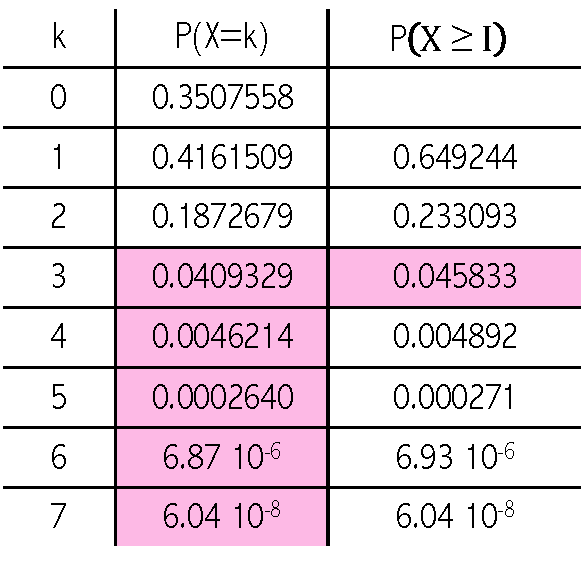
\includegraphics[width=0.3\textwidth]{extrem/TabExt.pdf}
\caption{Wahrscheinlichkeit $P(X = k))$ aller Ereignisse unseres Beispiels und die Wahrscheinlichkeiten $P(X \ge I)$ der komplementären Verteilfunktion. Die Rosa markierten Felder sind die Werte welche zur Berechnung in XX gebraucht wurden. }
\label{TabExt}
\end{figure}

\begin{figure}
\centering
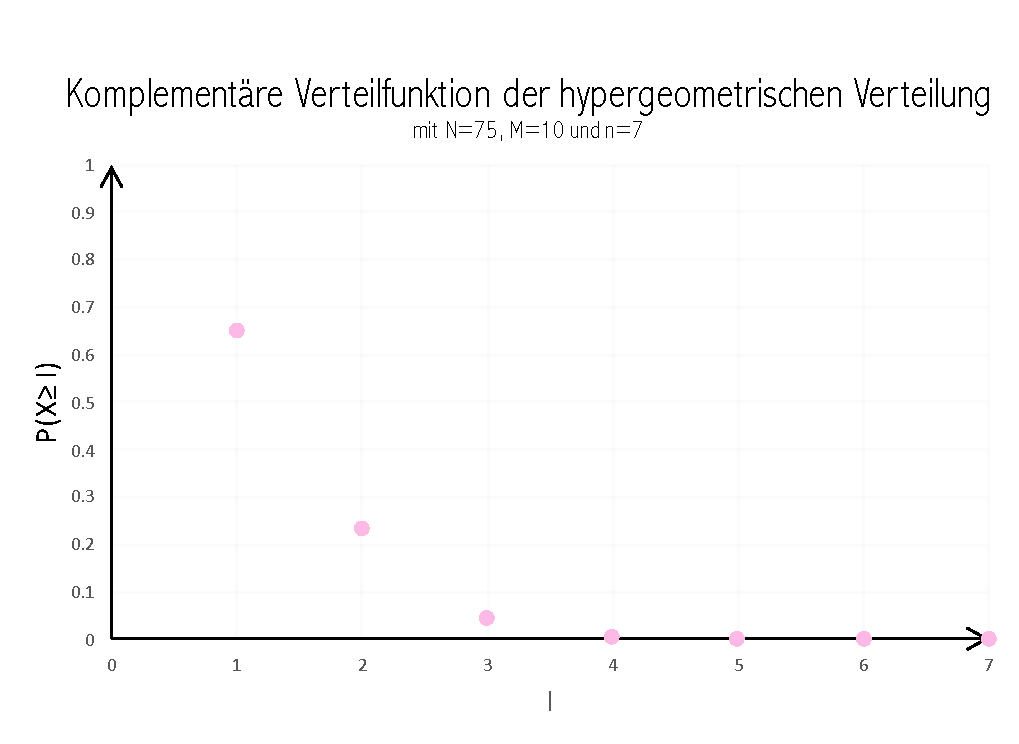
\includegraphics[width=0.8\textwidth]{extrem/HyperExt.pdf}
\caption{Die komplementäre Verteilfunktion $\bar{F}(x)$ der hypergeometrischen Verteilung zeigt auf, wie wahrscheinlich es ist mehr als k Ereignisse in den letzten 10 Jahren vorzufinden.}
\label{HyperExt}
\end{figure}



\section{Hypothesentest}
Hypothesentests werden immer dann durchgeführt, wenn aus erhobenen Daten etwas nachgewiesen werden muss, zum Beispiel das sich extreme Ereignisse in den letzten Jahren häufen. Der Grundsatz bei allen statistischen Tests ist, das wir das Gegenteil widerlegen müssen - wir müssen also widerlegen, dass extreme Ereignisse in den letzten Jahren zufällig verteilt sind. Das heisst die Häufung von extremen Ereignissen entscheidet der Zufall und werden nicht beeinflusst.

Zu vergleichen ist ein Hypothesentest mit einer Gerichtsverhandlung. Den im Zweifel ist das Gericht immer für den Angeklagten. Es muss davon ausgegangen werden, dass die Hypothese stimmt, bis das Gegenteil bewiesen werden kann. Hierfür benötigt es genügend Beweise, welche die Schuld oder hier die Hypothese widerlegen, ohne das Zweifel aufkommen können. Falls ungenügend viele Beweise vorliegen, muss davon ausgegangen werden, dass die Hypothese stimmt oder eben der Angeklagte unschuldig ist.
Zuerst wird die Nullhypothese aufgestellt, welche das Gegenteil von dem zu beweisenden Ziel aussagt.


\subsection{Nullhypothese}
Unsere Nullhypothese welche geprüft werden soll:

In den letzten Jahren gab es keinen Wandel oder eine Häufigkeit von extremen Ereignissen.
\begin{itemize}
\item Das Klima verändert sich nicht
\item Alles bleibt beim alten
\item Der Zufall bestimmt die Anordnung der (extremen) Ereignisse
\end{itemize}

Diese Nullhypothese gilt es nun zu widerlegen, um den Klimawandel zu beweisen.


\subsection{Signifikanzniveau}
Die Grenze für die Widerlegung der Nullhypothese beschreibt die statistische Signifikanz $\alpha$. Über diesen Wert wird eine bestimmte Irrtumswahrscheinlichkeit festgelegt.
Bei der Festlegung dieser Schwelle wird bedacht, was für Konsequenzen es hätte, dass ein beobachteter Unterschied nur zufällig erfolgt. Sind die Folgen gravierend, wählt man eher ein tiefes Niveau (1 \% statt 5\%).Bei einem Medikament wird daher eher ein tiefes Signifikanzniveau gewählt. Als Vergleich, beim Nachweis der Existenz des Higgs-Bosons\footnote{%
Das Higgs-Boson ist Elementarteilchen (Benannt nach dem britischen Physiker Peter Higgs), deren Existenz wurde im Juli 2012 durch das CERN (mit dem Larce Hadron Collider LHC) bestätigt.} wurde ein noch viel strengeres Kriterium gewählt, es entspricht einem Wert von 1 in 3.5 Millionen. 

Da extreme Ereignisse nicht direkt Lebensbedrohlich sind, wird im Folgenden $\alpha$ = 5\% gewählt.
Falls die Nullhypothese richtig ist, darf die Wahrscheinlichkeit dafür, dass sie fälschlicherweise abgelehnt wird, nicht unter 5\% fallen (Abbildung \ref{SigniAlpha}).


Eine Häufung von 3 oder mehr extremen Ereignissen wären nicht mehr durch den Zufall bestimmt. Das bedeutet, wenn von den 7 extremsten Ereignissen der letzten 75 Jahre 3 oder mehr in den letzten 10 Jahren waren, müssen wir auf den Klimawandel schliessen. Die Nullhypothese wäre ohne Zweifel widerlegt.

\begin{figure}
\centering
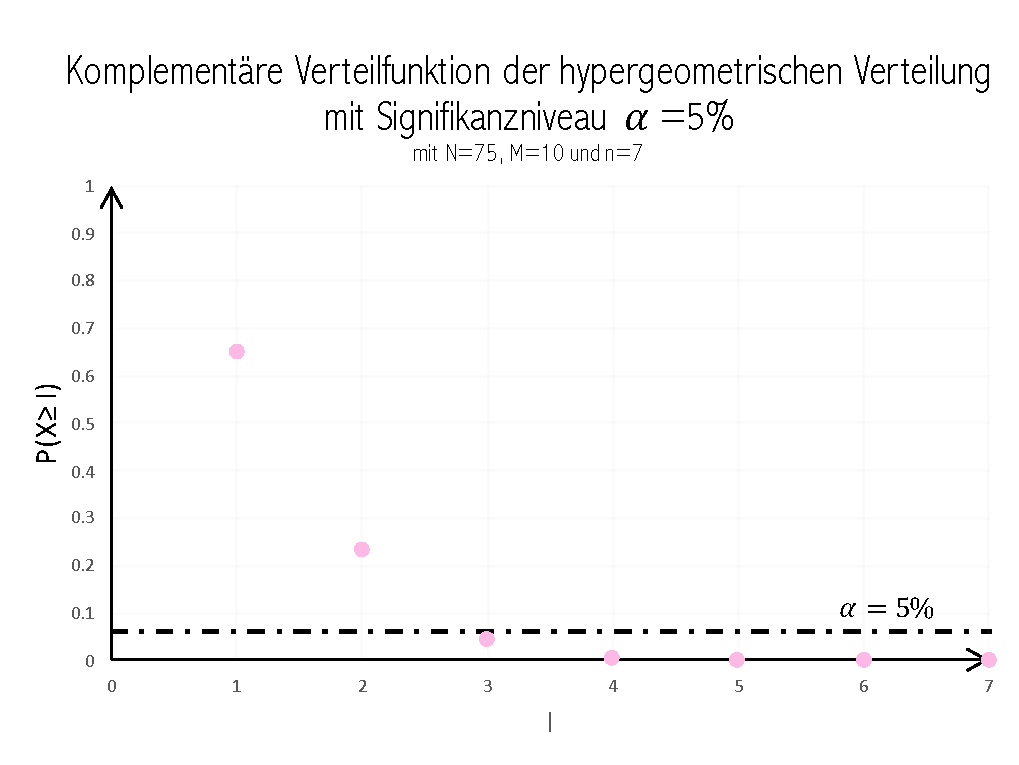
\includegraphics[width=0.8\textwidth]{extrem/SigniAlpha.pdf}
\caption{Die komplementäre Verteilfunktion der hypergeometrischen Verteilung mit dem eingezeichneten Signifikanzniveau von.}
\label{SigniAlpha}
\end{figure}


\section{Messpunkte Schweiz} \label{MesspunkteSchweiz}
Um eine möglichst grosse Vielfalt von Messreihen zu bekommen, werden verschiedene Messpunkte in der Schweiz \ref{MesspunkteCH}) angeschaut. 

\begin{figure}
\centering
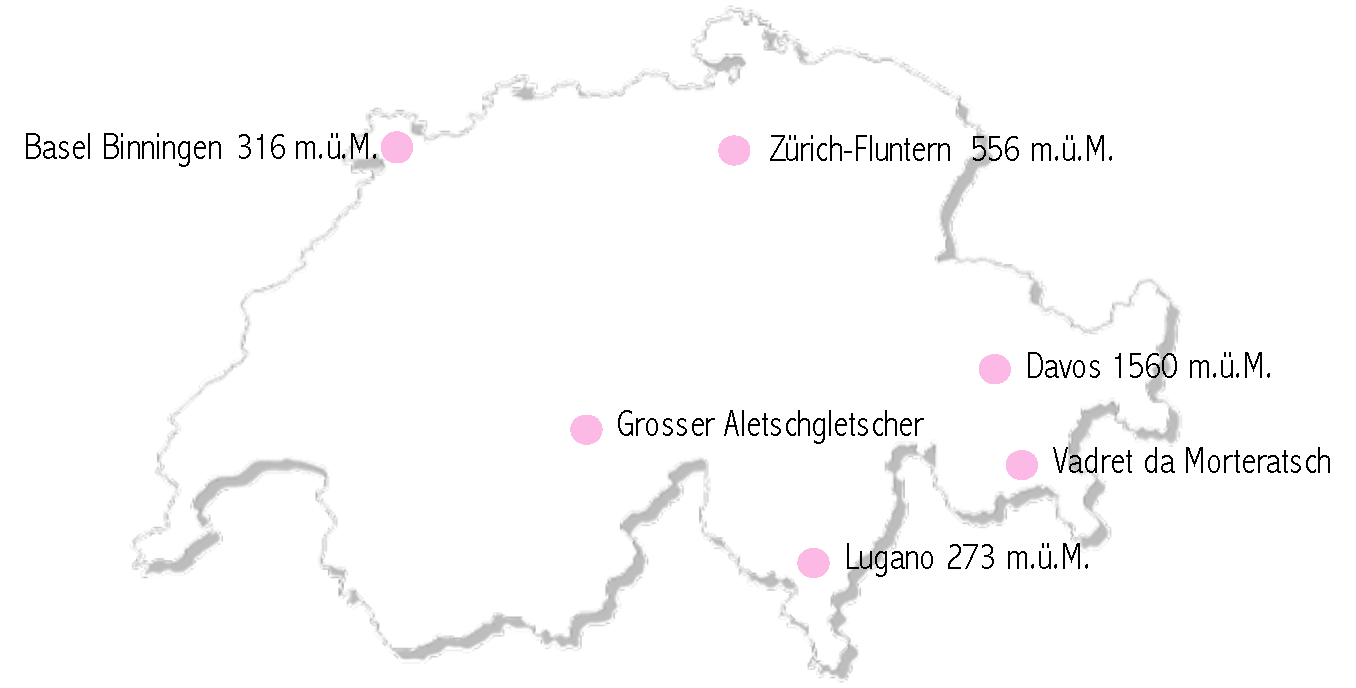
\includegraphics[width=0.8\textwidth]{extrem/Schweiz.pdf}
\caption{Gewählte Messpunkte in der Schweiz.}
\label{MesspunkteCH}
\end{figure}

Die Messreihen der Standorte Basel Binningen, Zürich-Fluntern, Lugano und Davos sind von MeteoSchweiz und sind öffentlich zugänglich. Die Daten sind bereits homogenisiert.
Die Messdaten der Gletscher werden vom Schweizerischen Gletschermessnetz GLAMOS \footnote{%
Die Veränderungen der Schweizer Gletscher werden jährlich gemessen. Das Messnetz GLAMOS wird getragen durch die ETH Zürich und die Universitäten Fribourg und Zürich mit finanzieller Unterstützung durch das Bundesamt für Umwelt BAFU, MeteoSchweiz und SCNAT.} ebenfalls öffentlich zugänglich zur Verfügung gestellt.


\subsection{Prüfung Messreihe}
Die Messreihen geben einen Einblick über die letzten 75 Jahre, nämlich von 1943 -- 2017. Damit die Hypothese widerlegt wird und somit der Klimawandel nachgewiesen werden kann, müssen drei oder mehr extreme Ereignisse in den letzten 10 Jahren vorkommen (Abbildung \ref{TabExt}). Das Signifikanzniveau $\alpha = 5\%$ wird unterschritten \ref{SigniAlpha}) und die Hypothese ohne jegliche Zweifel widerlegt.
Die detaillierten Auswertungen der Messreihen und Gletscherdaten sind im Kapitel ~\ref{AuswertungKG} \nameref{AuswertungKG} aufgeführt.


\section{Temperatur}
Die Jahresmitteltemperatur in der Schweiz ist seit 1864 rund $2^{\circ}$ gestiegen (Stand 2018, MeteoSchweiz). Der grösste Anstieg passierte in den letzten Jahrzehnnten. Dennoch ist für die breite Bevölkerung ein Anstieg von $2^{\circ}$ schwierig nachzuvollziehen.
In den nachfolgenden Beispielen, wurden Klimaindikatoren gewählt, welche jeder kennt, spürbar sind und beobachtet werden können.

\subsection{Jahres Mitteltemperatur}
Die Jahres Mitteltemperatur ist wie folgt definiert

\begin{definition}
Mittlere Jahrestemperatur in $^{\circ}$C.
\end{definition}

Bei der Jahresmitteltemperatur ist das Ergebnis eindeutig (Abbildung \ref{JMittel}). Bei beiden Messpunkten, sowohl Lugano als auch Basel Binningen, wird der Hypothesentest widerlegt da die Alphagrenze deutlich unterschritten wird. Bei Basel Binningen kommen vier der extremsten Ereignisse in den letzten 10 Jahren vor. In Lugano sind es sogar deren fünf! Der Klimawandel ist ohne jeden Zweifel nachgewiesen.


\subsection{Sommertage}
Ein Sommertag ist wie folgt definiert

\begin{definition}
Maximale Temperatur $\ge 25^{\circ}$C und langjähriger Mittelwert (1961 - 1990).
\end{definition}

Die Sommertage in Lugano waren in den letzten 10 Jahren nie extrem (Abbildung \ref{Sommertage}). Zu Beginn der Messungen in den 40er und 50er Jahren, zeigen sich Extremwerte. Wohingegen Davos eine Häufung der Anzahl von Sommertagen in den letzten 10 Jahren zeigt. In den früheren Messjahren waren keine oder nur sehr wenige Sommertage vorhanden. In den letzten 10 Jahren ist die Anzahl der Sommertage aber immer weiter gestiegen und mit 5 Ereignissen eigentlich nahezu unmöglich. In Davos wird die Hypothese widerlegt und somit ein Wandel im Klima nachgewiesen.


\subsection{Tropennächte}
Eine Tropennacht ist wie folgt definiert

\begin{definition}
Minimale Temperatur $\ge 20^{\circ}$C und langjähriger Mittelwert (1961 -- 1990).
\end{definition}

Sowohl in Lugano wie auch Basel Binningen sind in den letzten 10 Jahren eine extreme Anzahl von Tropennächten gemessen worden (Abbildung \ref{Tropennacht}). Mit vier Ereignissen pro Standort wird das Signifikanzniveau deutlich unterschritten, wie in denn vorangegangenen Messreihen Jahres Mitteltemperatur und Sommertage ist der Klimawandel real und nachgewiesen.


\subsection{Hitzetage}

Ein Hitzetag ist wie folgt definiert

\begin{definition}
Maximale Temperatur $\ge 30^{\circ}$C und langjähriger Mittelwert (1961 -- 1990).
\end{definition}

Bei den Hitzetagen ist im Klima kein Wandel zu erkennen (Abbildung \ref{Hitzetage}). Weder in Zürich-Fluntern noch in Lugano wurden in den letzten Jahren extrem viele Hitzetage gemessen. Bei beiden Orten, waren Hitzetage zu Beginn der Messreihen in den 40er Jahren häufiger.


\subsection{Frosttage}
Ein Frosttag ist wie folgt definiert

\begin{definition}
Minimale Temperatur $< 0^{\circ}$C und langjähriger Mittelwert (1961 -- 1990).
\end{definition}

Wie bereits bei den Hitzetagen ist auch bei den Frosttagen weder in Basel Binningen noch in Lugano kein Wandel im Klima zu erkennen (Abbildung \ref{Frosttage}). Ebenso wurden die Extremen vermehrt zu Beginn der Messreihe gemessen.


\subsection{Eistage}
Ein Eistag ist wie folgt definiert

\begin{definition}
Maximale Temperatur $< 0^{\circ}$C und langjähriger Mittelwert (1961 -- 1990).
\end{definition}

Anhand der Anzahl Eistage in Zürich-Fluntern und Davos, kann kein Klimawandel festgestellt werden (Abbildung \ref{Eistage}). Weder in den oberen noch in den unteren Extremen. 


\section{Niederschlag}
In den letzen Jahren nahmen die Niederschläge zu. Die Schadensumme der Hochwasserereignisse in der Schweiz beläuft sich durchschnittlich auf 300 Millionen Schweizer Franken pro Jahr. Vor allem im Jahr 2005 kam es zu extremen Hochwasserereignissen infolge starker Unwetter welche über die Schweiz zogen. Ausuferungen, Überschwemmungen und Schlammlawinen waren Folgen von diesen heftigen Unwetter. Die Schadensumme belief sich auf 3 Milliarden Schweizer Franken. 


\subsection{Jahresniederschlag}
Der Jahresniederschlag ist wie folgt definiert

\begin{definition}
Jahresniederschlag in mm.
\end{definition}

Der Jahresniederschlag hat in den letzten Jahren zwar zugenommen, zeigt aber keine Häufung von extremen Ereignissen in den letzten 10 Jahren (Abbildung \ref{Jahresniederschlag}). Anhand des Jahresniederschlag kann man nicht auf den Klimawandel schliessen. Hier wäre es interessant eine Messereihe zu testen, welche die Anzahl Starkniederschläge pro Jahr aufzeigt.


\subsection{Neuschnee}
Die Neuschneemenge ist wie folgt definiert

\begin{definition}
Neuschneemenge, Jahressumme der täglichen Aufzeichnung in cm.
\end{definition}

Ähnlich sieht es bei der Neuschneemenge aus (Abbildung \ref{Neuschnee}). Weder bei extrem viel gefallenem Neuschnee, noch bei extrem wenig gefallenem Neuschnee ist ein Klimawandel zu erkennen. Hier wäre ebenfalls die Fragestellung anzupassen und abzuändern in: Wie lange bleibt der Neuschnee liegen?


\section{Gletscher}
Bei den Gletscherdaten wurde der Zeitraum von 1881 -- 2017 gewählt. Durch die höhere Anzahl an Messjahren, müssen die Wahrscheinlichkeitswerte neu berechnet werden. Die Berechnungen ergeben leicht veränderte Werte, es müssen aber ebenso 3 oder mehr extreme Ereignisse in den letzten 10 Jahren vorkommen um diese dem Klimawandel zuschreiben zu können.


\subsection{Grosser Aletschgletscher}
Der grosse Aletschgletscher schmilzt, wie man gut auf der (Abbildung \ref{Aletsch}) sehen kann. Jedoch zeigen die Messwerte der letzen 136 Jahren keinen extremen Schwund der Eismassen auf.

Anhand der Messdaten ist kein Klimawandel nachweisbar (Abbildung \ref{AletschTab}). Hier müsste allerdings die Messreihe hinterfragt werden. Die Messreihe zeigt nur die Längenänderung pro Jahr wieviel die Gletscherzunge schwindet und nicht die Volumenänderung der Eismasse. Der Gletscher könnte in der Länge nur wenig schwinden würde aber im selben Jahr sehr viel an Volumen verlieren, wäre dies dennoch nicht in der Messreihe ersichtlich.


\subsection{Vadret da Morteratsch}
Beim Morteratschgletscher sieht es anders aus. Die Längenänderung in den letzten 10 Jahren ist massiv (Abbildung \ref{Morteratschtab}). Hier kann aufgrund der extremen Längenänderung auf den Klimawandel geschlossen werden. Dies ist auch deutlich in der (Abbildung \ref{Morteratsch}) ersichtlich. Speziell in diesem Fall, wäre es spannend ob die Abnahme des Eisvolumens ebenso auf den Klimawandel schliessen würde oder nicht.





\section{Ist die Klimawandel in der Schweiz real?}
Diese Methode liefert schnell und einfach ein Ergebnis ob ein Wandel in einer Klimamessreihe dem Klimawandel zugeschrieben werden kann oder ob es sich um eine zufällige Häufung von extremen Ereignissen handelt. Aus den analysierten Klimaindikatoren ist der Klimawandel nicht immer eindeutig hervorgegangen (Abbildung \ref{AuswertungK}). 

\begin{figure}
\centering
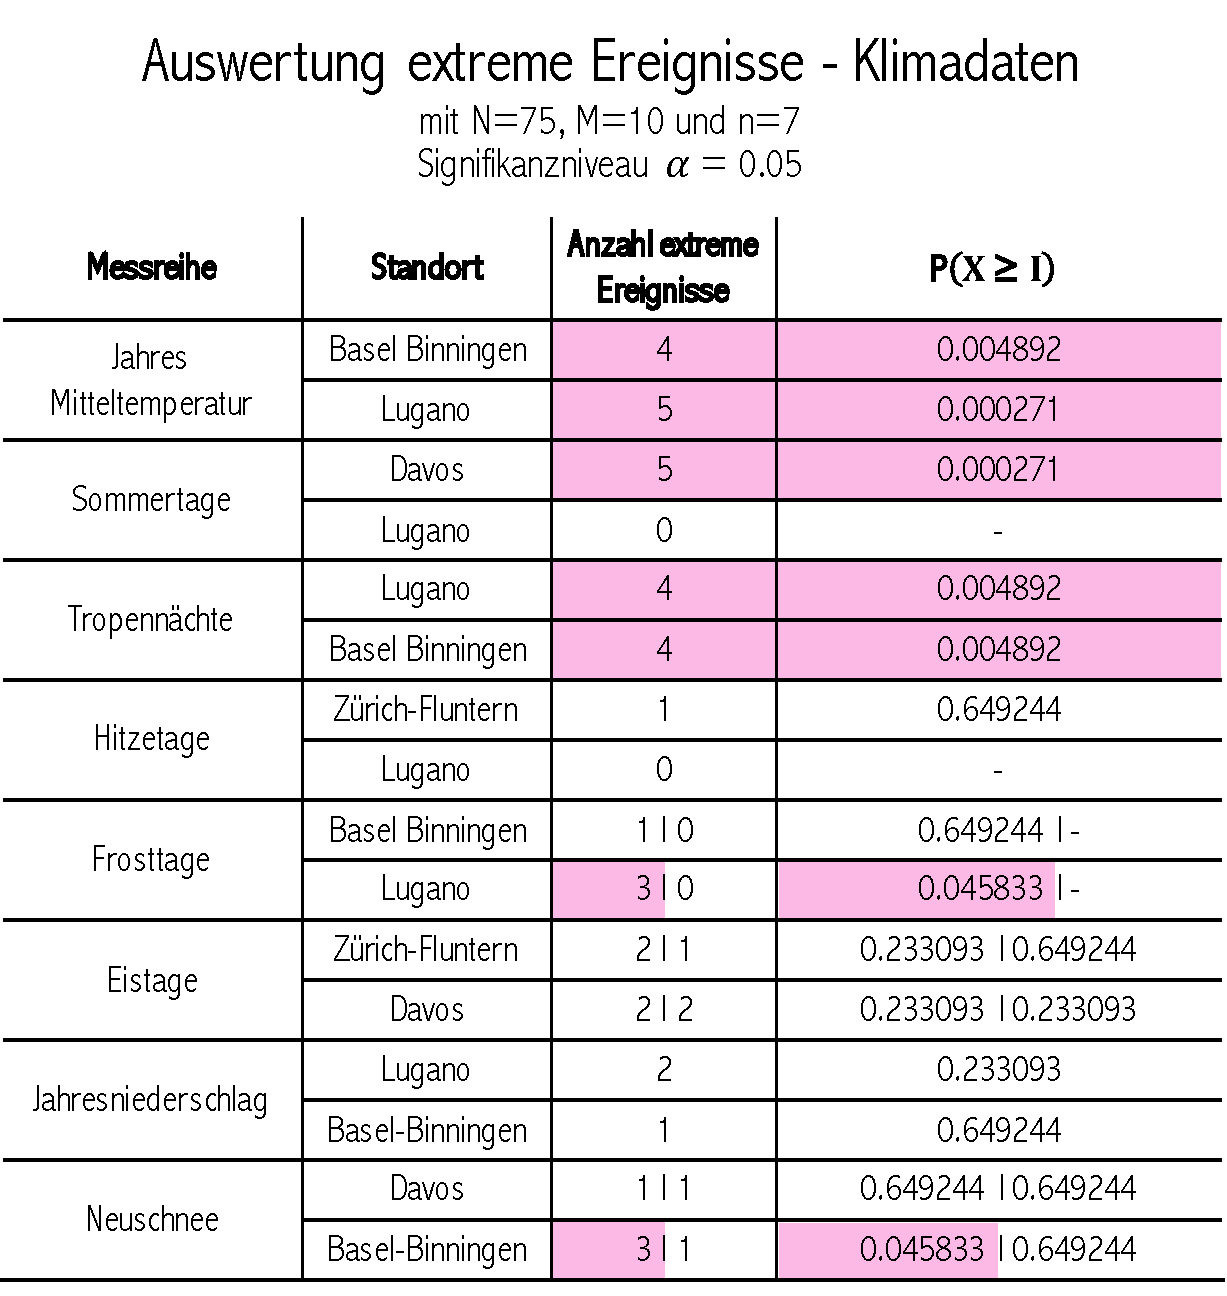
\includegraphics[width=0.7\textwidth]{extrem/AuswertungK.pdf}
\caption{Die Auswertung der Klimadaten schafft einen Überblick, welche Klimaindikatoren vom Klimawandel betroffen sind und welche nicht. Rosa markiert sind jene, welche das Signifikanzniveau $\alpha=0.05$ unterschreiten. Die Häufung jener extremen Ereignisse (in den letzten 10 Jahren), ist dem Klimawandel zuzuschreiben.}
\label{AuswertungK}
\end{figure}


\begin{figure}
\centering
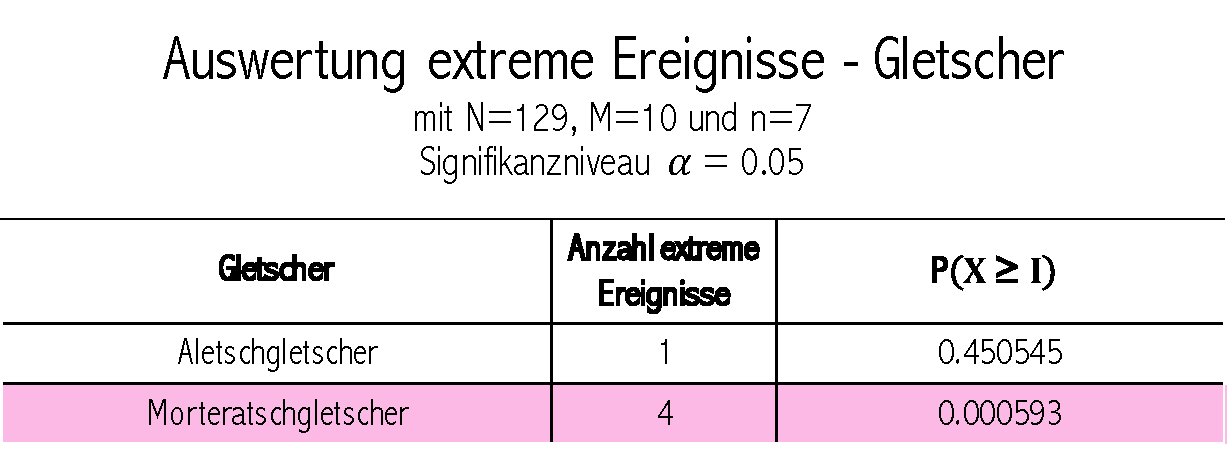
\includegraphics[width=0.7\textwidth]{extrem/AuswertungG.pdf}
\caption{Die Auswertung der Gletscherdaten schafft ebenso einen Überblick über die beiden Gletscher ob diese vom Klimawandel betroffen sind oder nicht.}
\label{AuswertungG}
\end{figure}

Dennoch lässt sich die Frage ob der Klimawandel in der Schweiz real ist deutlich mit $\flqq Ja \frqq$ beantworten. Vor allem die Indikatoren rund um die Temperatur zeigen einen deutlichen Wandel. Besonders die Jahres Mitteltemperatur, Tropennächte und die Sommertage weisen eine starke Veränderung im Vergleich zur Vergangenheit auf. Wohingegen bei den Niederschlägen und teilweise auch Gletschern (Abbildung \ref{AuswertungG}). kein Klimawandel festgestellt werden konnte. Mit den Vorschlägen zur Untersuchung von weiteren und anders formulierten Messreihen könnte ein Wandel eventuell auch noch bei anderen Klimaindikatoren und Messreihen aufgezeigt werden.

Mit dieser Berechnungsweise lässt es sich ohne Vorurteile und Einflüsse neutral bewerten ob der Klimawandel vorhanden ist oder nicht. Aufgrund der Tatsache, dass von acht getesteten Klimaindikatoren, fünf die Hypothese widerlegen, kann davon ausgegangen werden, dass der Klimawandel real ist. Das Klima ändert sich, ob dies gut oder schlecht für die Menschheit ist wird sich in der Zukunft zeigen. Feststeht das die Erde auch dieses extreme Ereignis wie den Klimawandel überstehen wird - mit oder ohne uns, dass liegt in unseren Händen.


\section{Auswertung der Klima- und Gletscherdaten} \label{AuswertungKG}

\begin{figure}
\centering
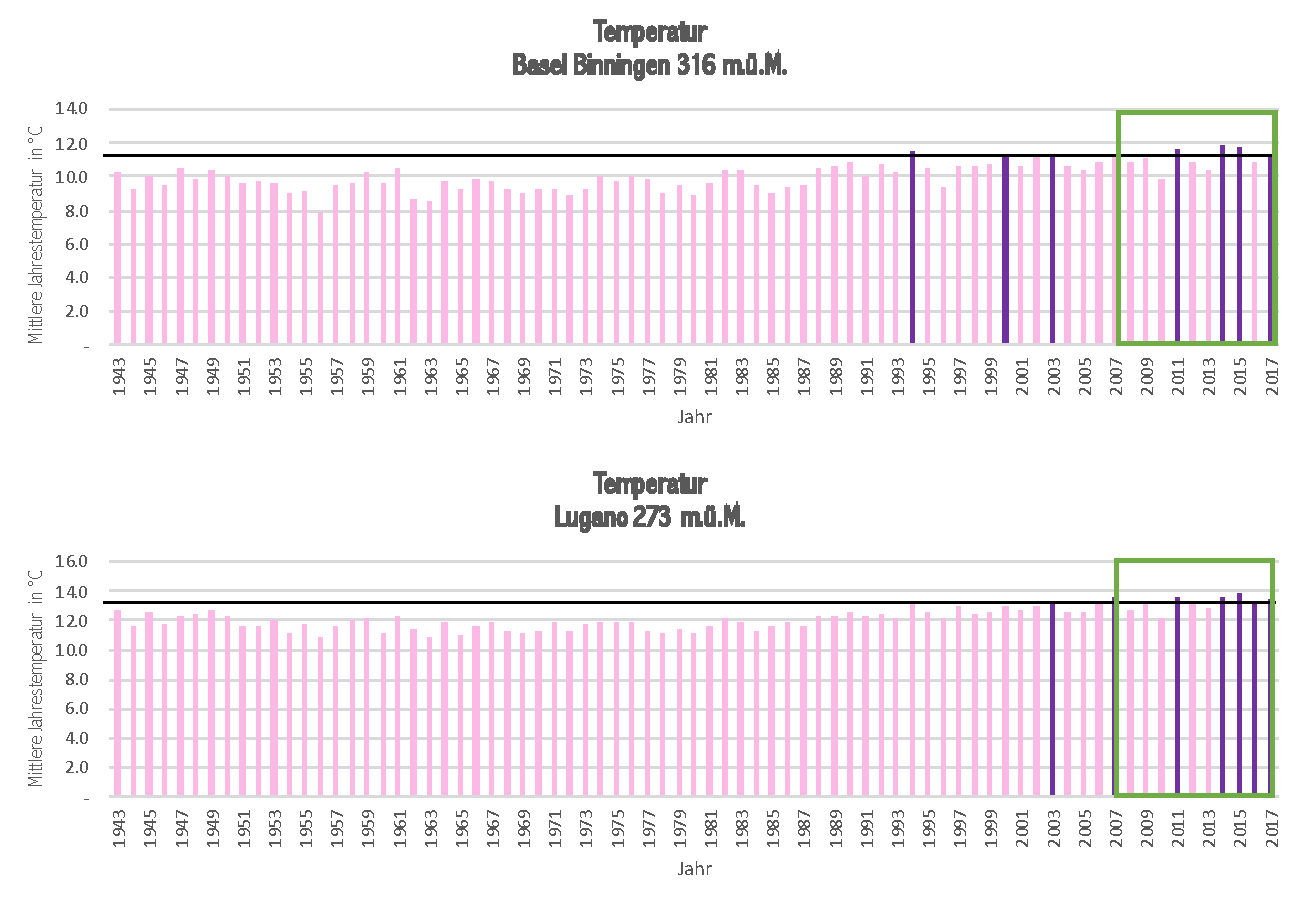
\includegraphics[width=0.8\textwidth]{extrem/JahresMittel.pdf}
\caption{Die Jahres Mitteltemperatur der beiden Standorte Basel Binningen und Lugano. Bei beiden Standorten wird das Signifikanzniveau deutlich unterschritten und der Klimawandel ist nachgewiesen.}
\label{JMittel}
\end{figure}


\begin{figure}
\centering
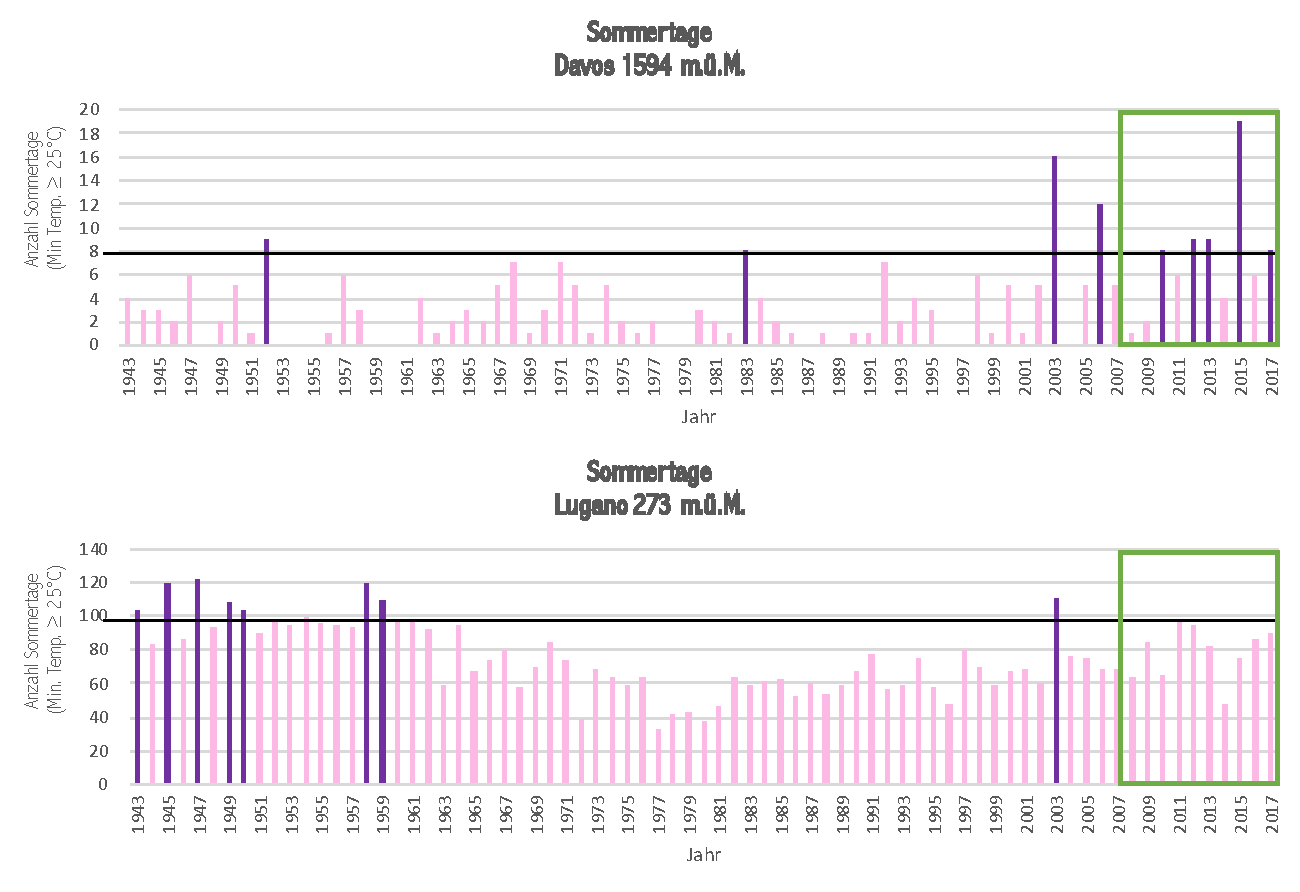
\includegraphics[width=0.8\textwidth]{extrem/Sommertage.pdf}
\caption{Die Anzahl Sommertage im Verlauf der Messreihe an den Standorten Davos und Lugano. Beim Standort Davos kann der Klimawandel nachgewiesen werden, 5 extreme Ereignisse in den letzten 10 Jahren stattgefunden haben.}
\label{Sommertage}
\end{figure}


\begin{figure}
\centering
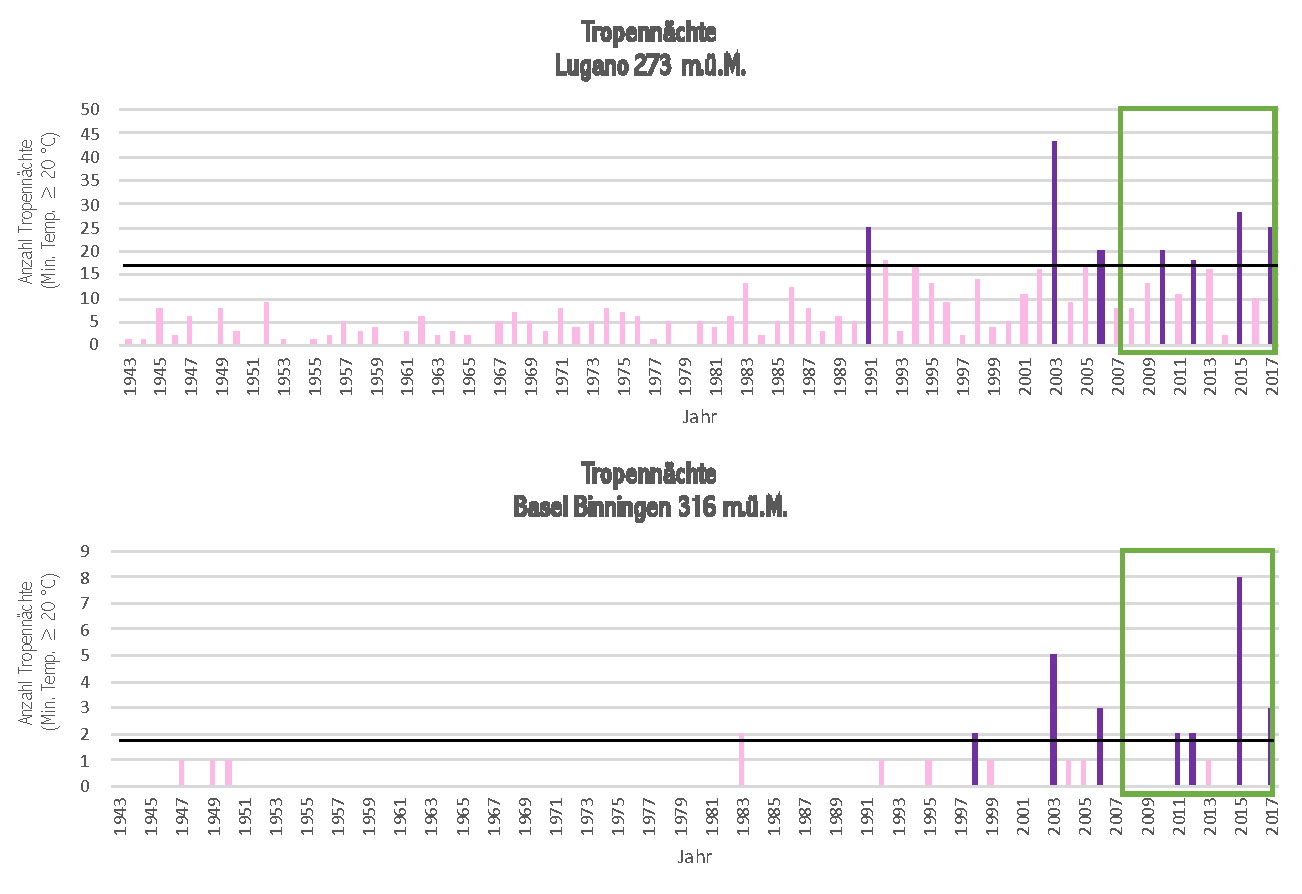
\includegraphics[width=0.8\textwidth]{extrem/Tropennacht.pdf}
\caption{Die Anzahl Tropennächte an den Standorten Basel Binningen und Lugano in den vergangenen Jahren. Bei beiden Standorten wird der Klimawandel nachgewiesen.}
\label{Tropennacht}
\end{figure}


\begin{figure}
\centering
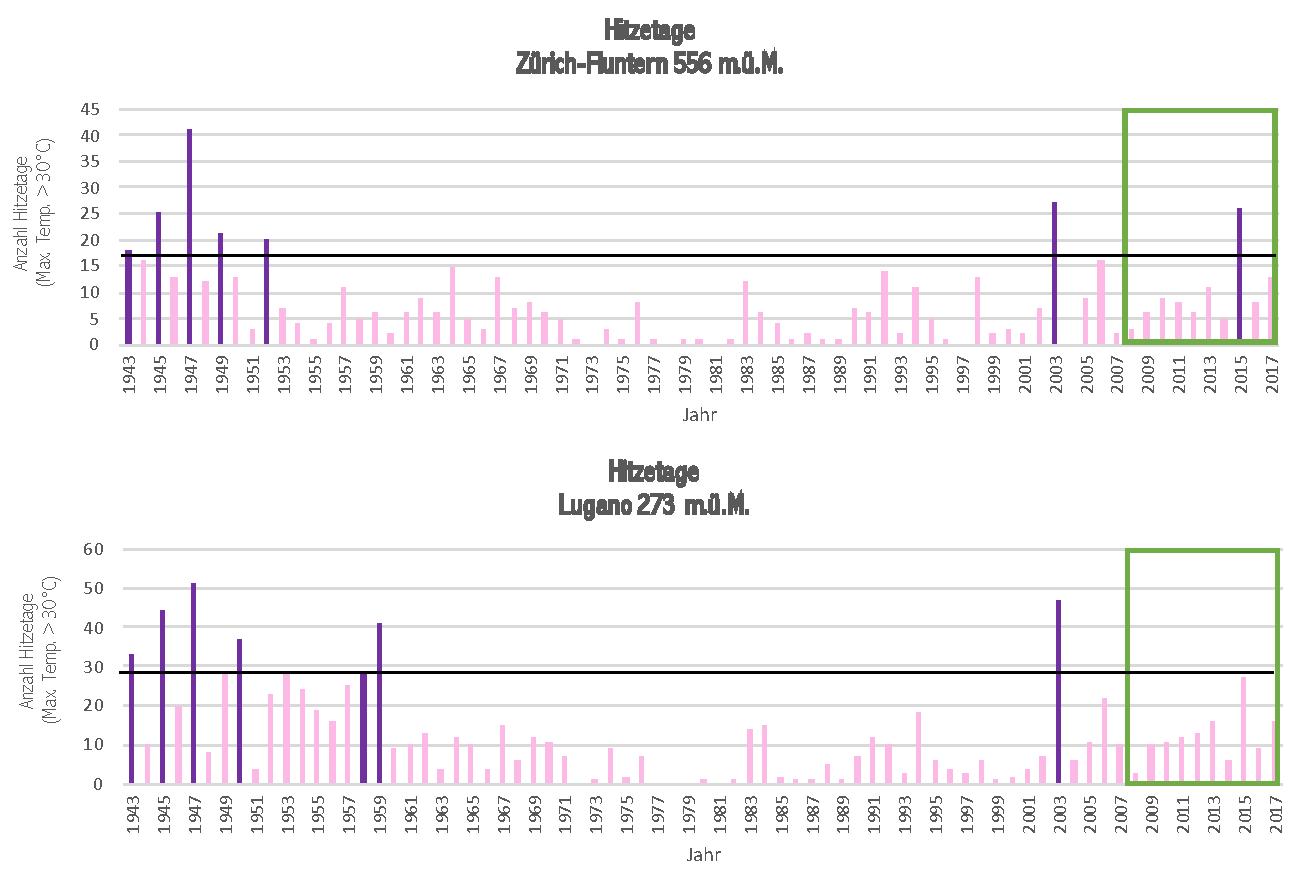
\includegraphics[width=0.8\textwidth]{extrem/Hitzetage.pdf}
\caption{Die Anzahl Hitzetage in der Messreihe an den Standorten Lugano und Zürich-Fluntern. Keine der beiden Standorte weisst anhand der Auswertung einen Klimawandel auf.}
\label{Hitzetage}
\end{figure}


\begin{figure}
\centering
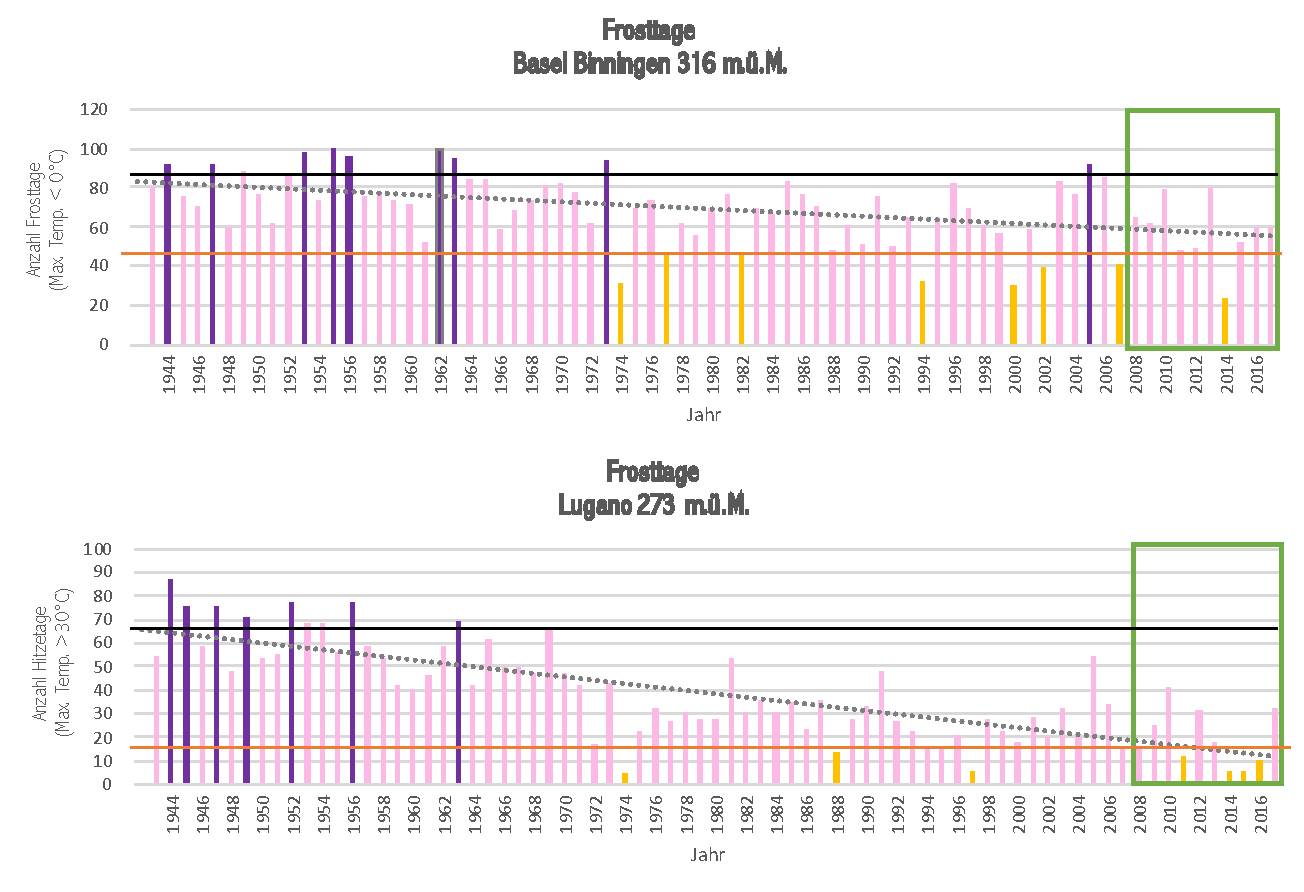
\includegraphics[width=0.8\textwidth]{extrem/Frosttage.pdf}
\caption{Die Anzahl Frosttage an den Standorten Lugano und Basel Binningen mit den oberen (violett) und unteren (gelb) Extremen Messwerten. Der Standort Lugano weisst mit den extrem wenigen Frosttagen einen Wandel im Klima auf.}
\label{Frosttage}
\end{figure}


\begin{figure}
\centering
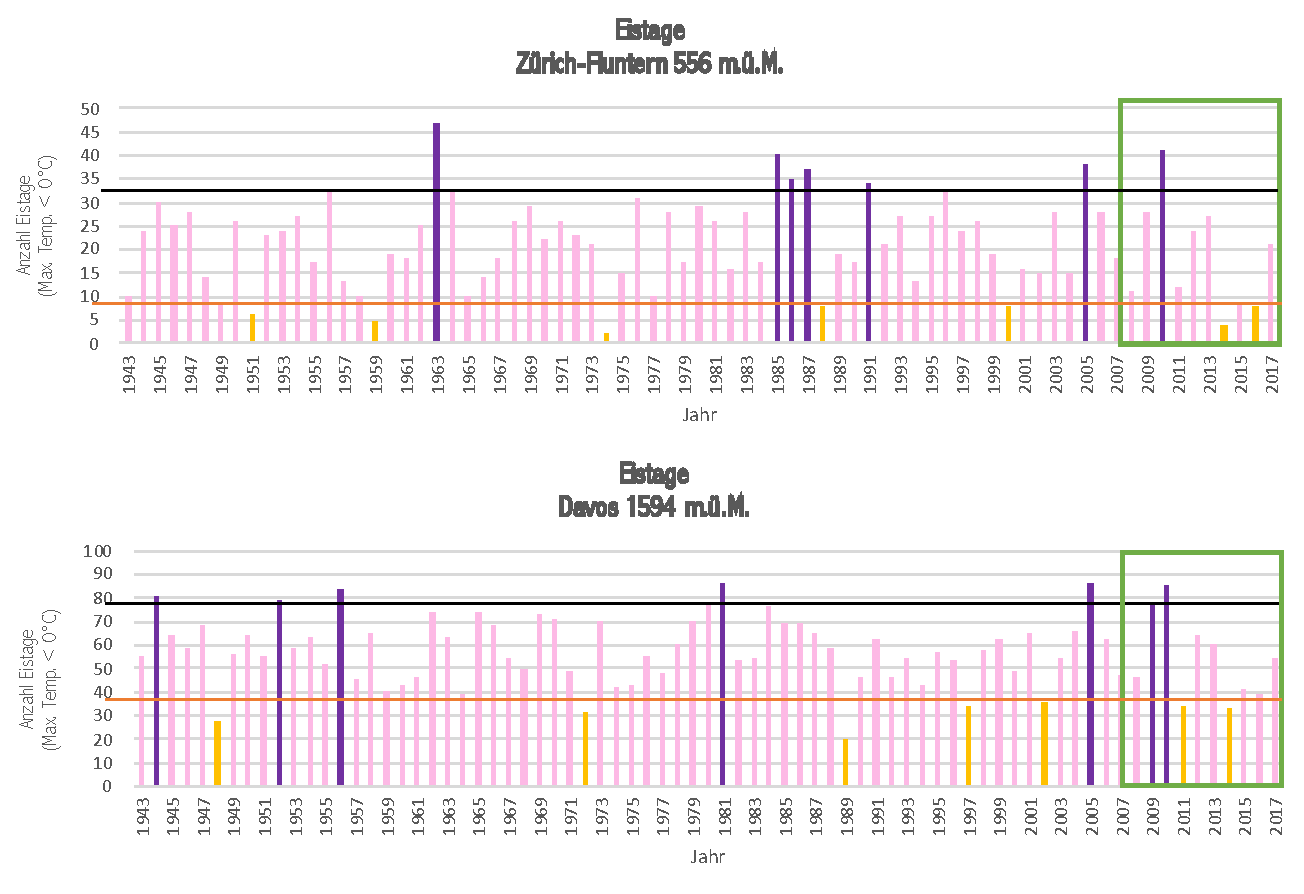
\includegraphics[width=0.8\textwidth]{extrem/Eistage.pdf}
\caption{Die Anzahl Eistage an den Standorten Zürich-Fluntern und Davos. Weder die obere (violett) noch die untere (gelb) extremen Ereignisse sind dem Klimawandel zuzuschreiben.}
\label{Eistage}
\end{figure}


\begin{figure}
\centering
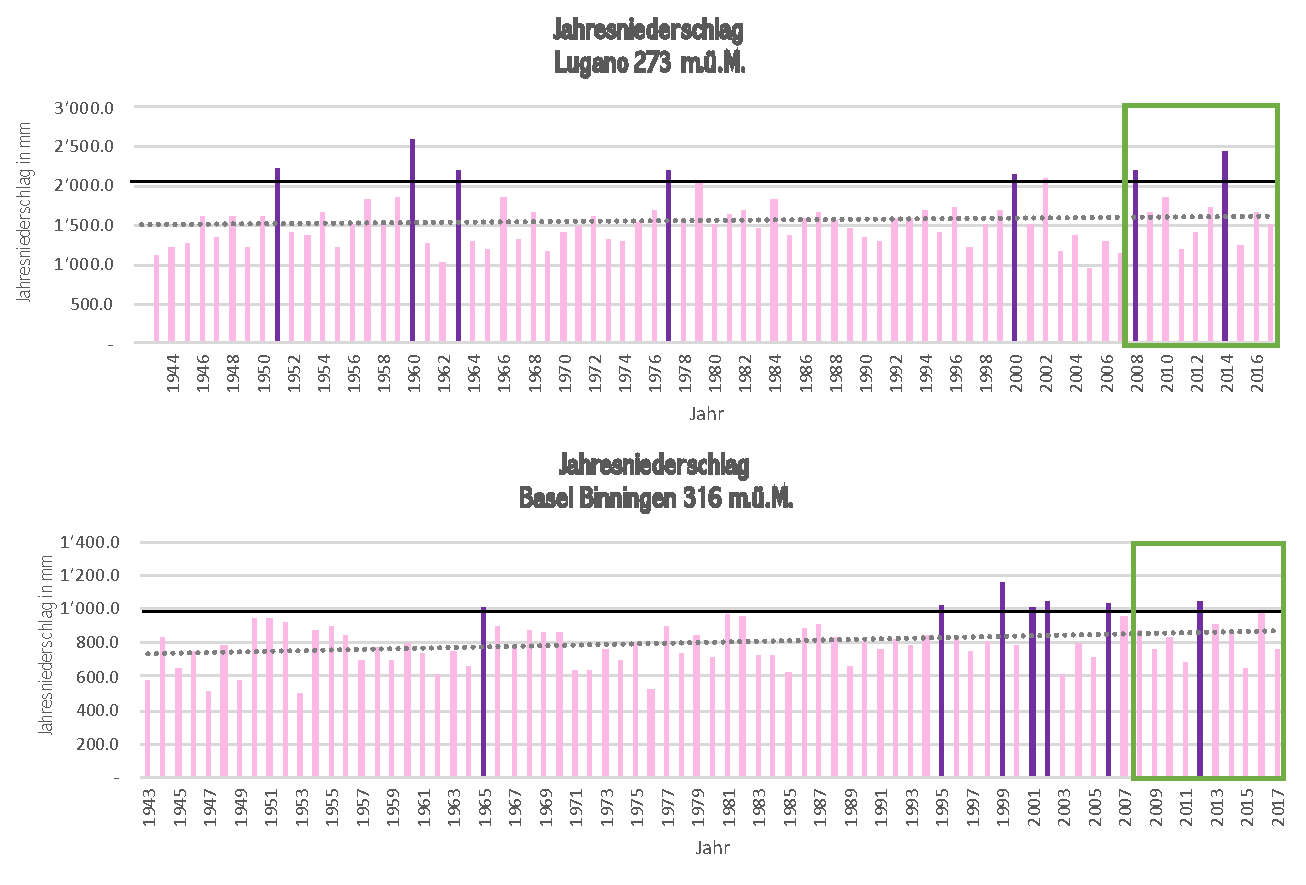
\includegraphics[width=0.8\textwidth]{extrem/Jahresniederschlag.pdf}
\caption{Der Jahresniederschlag gemessen in Millimeter pro Jahr. In den letzten 10 Jahren ist es nicht zu einer Häufung von extremen Ereignissen gekommen. Der Klimawandel wird nicht nachgewiesen.}
\label{Jahresniederschlag}
\end{figure}


\begin{figure}
\centering
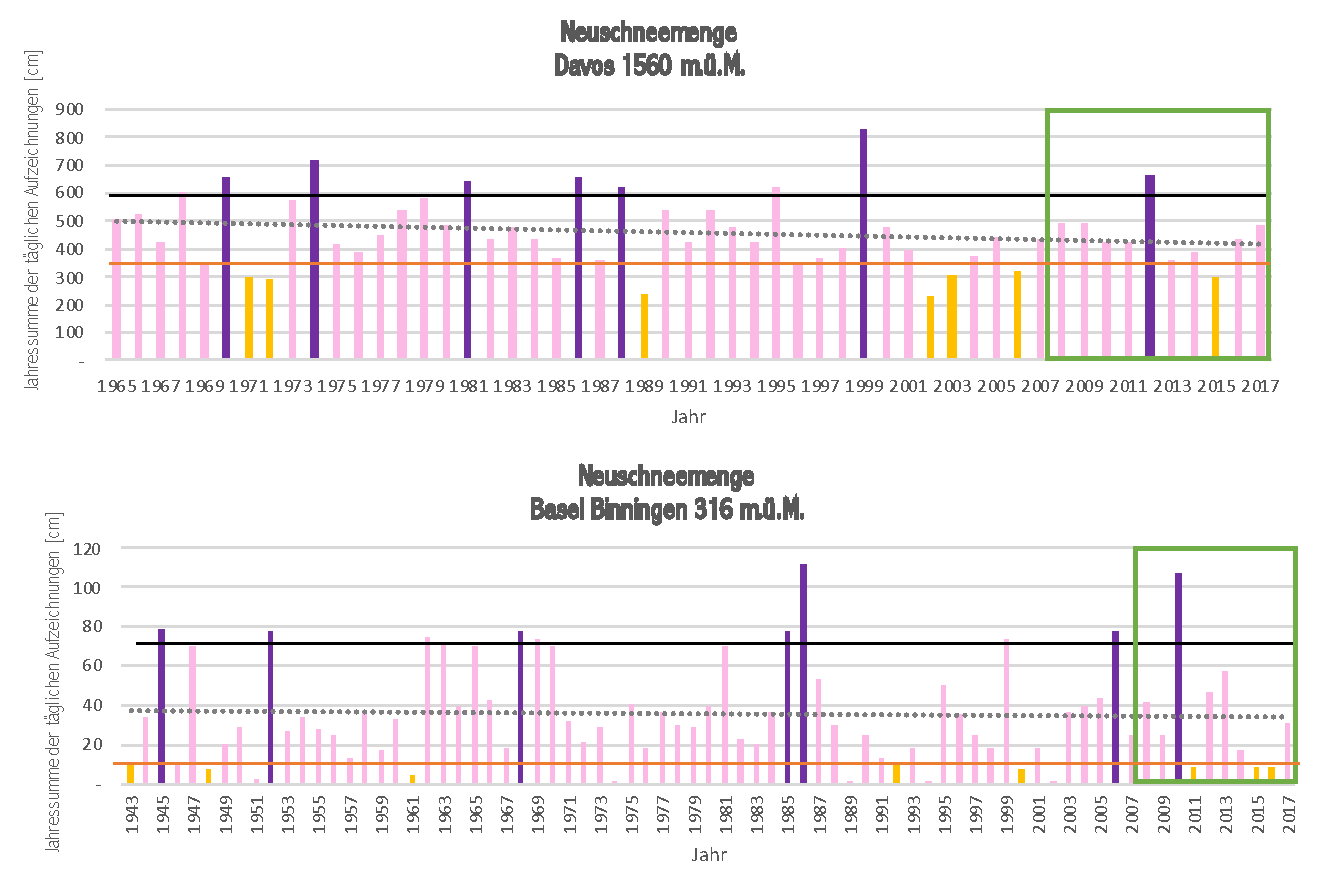
\includegraphics[width=0.8\textwidth]{extrem/Neuschnee.pdf}
\caption{Der Neuschnee gemessen in der Jahressumme an gefallenem Schnee, weisst wie der Jahresniederschlag keine Extremen in den letzten 10 Jahren auf, welche dem Klimawandel zugesprochen werden könnten.}
\label{Neuschnee}
\end{figure}


\begin{figure}
\centering
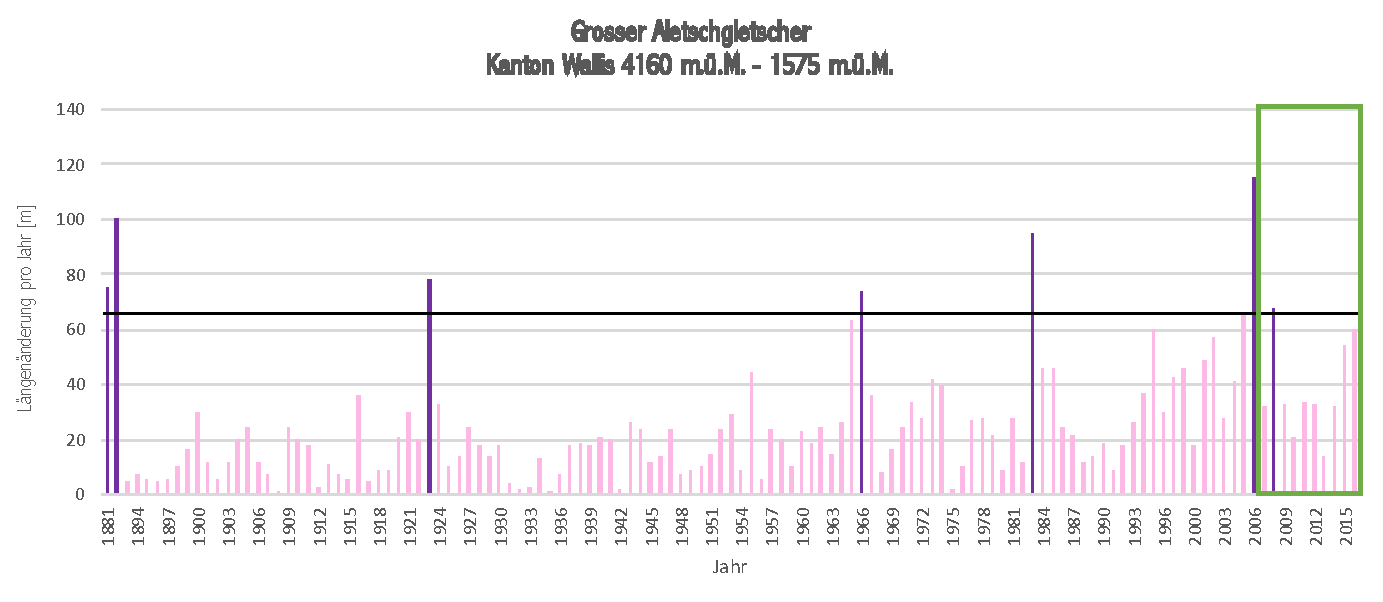
\includegraphics[width=1.0\textwidth]{extrem/Aletsch.pdf}
\caption{Die Längenänderung pro Jahr zeigt beim Aletschgletscher keine auffälligen oder gehäuften extreme Schmelzphasen. Somit kann kein Klimawandel nachgewiesen werden.}
\label{AletschTab}
\end{figure}


\begin{figure}
\centering
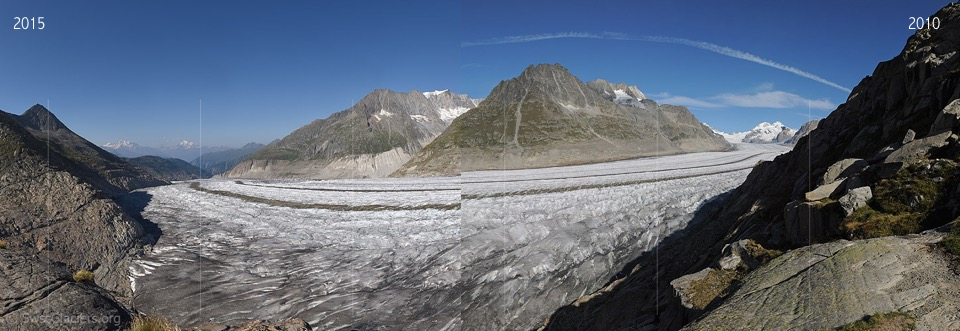
\includegraphics[width=1.0\textwidth]{extrem/Aletsch.jpg}
\caption{Der grosse Aletschgletscher im Wandel der Zeit. Links im Jahr 2015 und rechts im Jahr 2010. Die Volumenänderung ist deutlich ersichtlich.}
\label{Aletsch}
\end{figure}


\begin{figure}
\centering
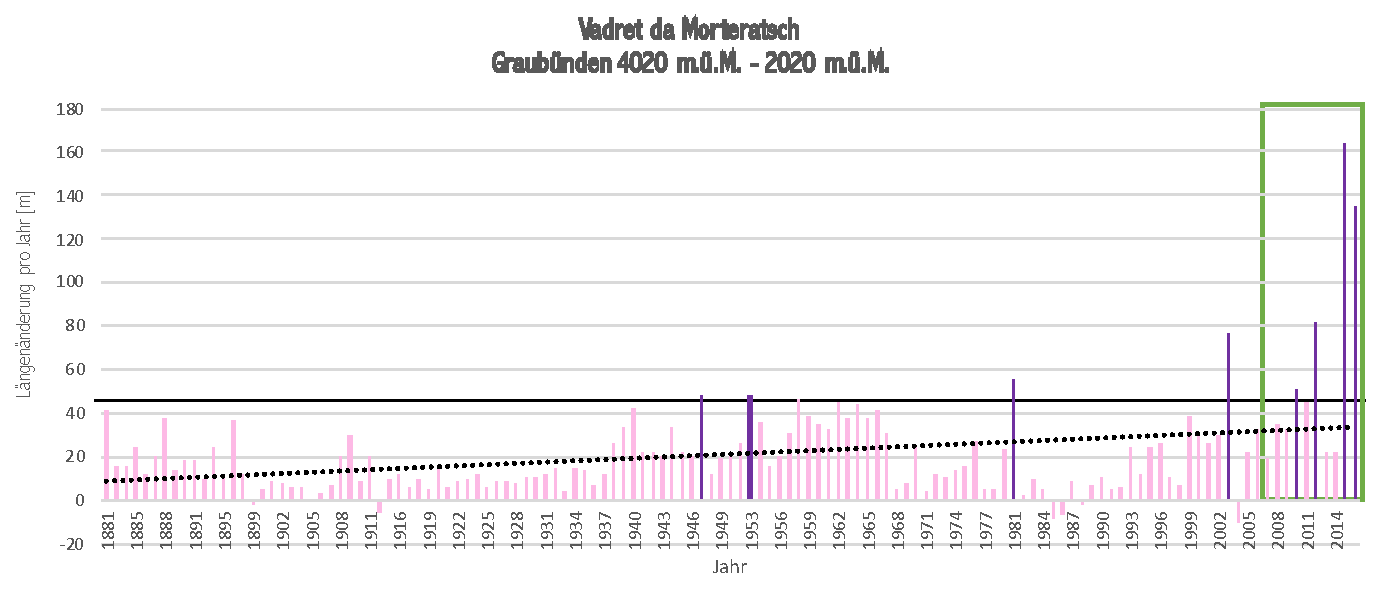
\includegraphics[width=1.0\textwidth]{extrem/Morteratsch.pdf}
\caption{Die Längenänderung pro Jahr zeigt beim Morteratschgletscher deutliche extreme Ereignisse auf. Der Einfluss auf die Längenänderung ist ganz deutlich dem Klimawandel zuzuschreiben. Bemerkenswert ist das Jahr 2004, denn der Morteratschgletscher ist in diesem Jahr um 10 Meter gewachsen.}
\label{Morteratschtab}
\end{figure}


\begin{figure}
\centering
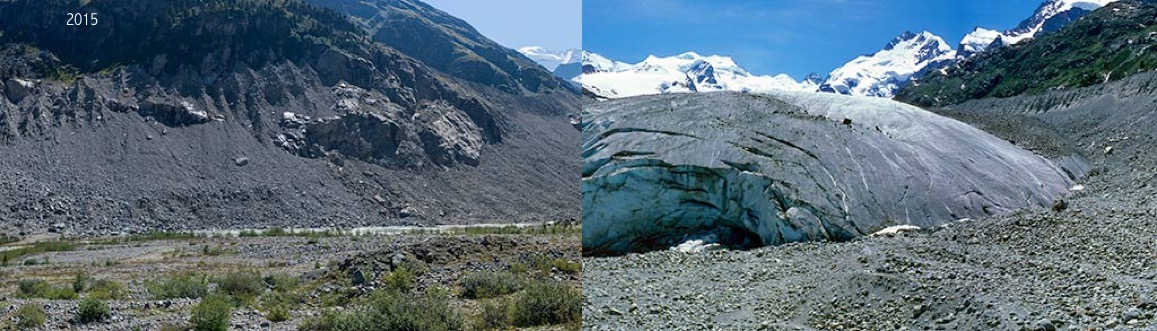
\includegraphics[width=1.0\textwidth]{extrem/Morteratsch.jpg}
\caption{Der Morteratschgletscher im Wandel der Zeit. Links im Jahr 2015 und rechts im Jahr 1985. Die starke Abnahme des Volumens und vor allem die Längenänderung ist unverkennbar.}
\label{Morteratsch}
\end{figure}



\rhead{Schlussfolgerung}


\rhead{Abschnitt}



\printbibliography[heading=subbibliography]
\end{refsection}
